\documentclass[11pt,a4paper]{article}
\usepackage[T1]{fontenc}
\usepackage[utf8]{inputenc}
\usepackage{lmodern}
\usepackage[margin=25mm,headheight=15pt]{geometry}
\usepackage{microtype}
\usepackage{amsmath,amssymb,amsthm,mathtools}
\usepackage{booktabs,array,longtable,tabularx}
\usepackage{graphicx,xcolor}
\usepackage{enumitem}
\usepackage{fancyhdr}
\usepackage{listings}
\usepackage[most]{tcolorbox}
\usepackage{hyperref}
\usepackage[nameinlink,noabbrev]{cleveref}
\definecolor{ink}{HTML}{163449}
\definecolor{teal}{HTML}{087F8C}
\definecolor{light}{HTML}{EEF5F7}
\hypersetup{colorlinks=true,linkcolor=ink,citecolor=teal,urlcolor=teal,
 pdftitle={Planar Canonical-Lift Diagrams and Reusable Sector Kernels for Unknot Recognition},
 pdfauthor={ProveIt research continuation}}
\newtheorem{theorem}{Theorem}[section]
\newtheorem{lemma}[theorem]{Lemma}
\newtheorem{proposition}[theorem]{Proposition}
\newtheorem{corollary}[theorem]{Corollary}
\theoremstyle{definition}
\newtheorem{definition}[theorem]{Definition}
\newtheorem{remark}[theorem]{Remark}
\newcommand{\R}{\mathbb R}
\newcommand{\Q}{\mathbb Q}
\newcommand{\N}{\mathbb N}
\newcommand{\poly}{\operatorname{poly}}
\newcommand{\basecommit}{8188525b70033dcfe7c51ea5ae2c8723ad0c0198}
\newcommand{\code}[1]{\texttt{\small #1}}
\setlist{itemsep=3pt,topsep=6pt}
\setlength{\parskip}{4pt}
\setlength{\parindent}{1.2em}
\setlength{\emergencystretch}{2em}
\linespread{1.04}
\pagestyle{fancy}
\fancyhf{}
\fancyhead[L]{\small\color{ink}ProveIt: planar normal sectors}
\fancyhead[R]{\small October 2026}
\fancyfoot[C]{\thepage}
\lstset{basicstyle=\ttfamily\footnotesize,breaklines=true,columns=fullflexible,
 frame=single,rulecolor=\color{light},backgroundcolor=\color{light},
 keepspaces=true,showstringspaces=false}

\begin{document}
\hypersetup{pageanchor=false}
\begin{titlepage}
\vspace*{0mm}
{\color{teal}\large PROVEIT RESEARCH CONTINUATION\par}
\vspace{8mm}
{\color{ink}\Huge\bfseries Planar Canonical-Lift Diagrams\par}
\vspace{3mm}
{\color{ink}\huge\bfseries and Reusable Sector Kernels\par}
\vspace{5mm}
{\color{ink}\Large for Unknot Recognition\par}
\vspace{8mm}
{\large Complete matching-dimension-three enumeration, independent
coverage certificates, and a growing geometric family\par}
\vspace{6mm}
{\normalsize Prepared for Vladimir Reshetnikov and the ProveIt project\\
October 2026\par}
\vspace{4mm}
\begin{abstract}
We extend the preceding minimum-envelope method from matching nullity at
most two to at most three.  For one supplied quadrilateral sector with
\(k\) allowed types, contraction of zero-labelled face equations leaves
at most \(8k\) triangle classes.  Its canonical standard-coordinate lift
is linear on the common refinement of planar minimum diagrams.  We prove
the explicit output bound
\[
 R\le b+2\sum_v(m_v-1)
       +9\sum_{v<w}(m_v-1)(m_w-1)=O(k^2),
\]
including degeneracies and a linear bound when only one vertex group
has a nontrivial diagram.  A simple exact implementation constructs all
rays in \(O(k^3+tk^2)\) scalar operations after matching elimination,
where \(t\) is the number of tetrahedra; integer normalization and bit
length are charged separately.  We also prove completeness of a compact
certificate based on dominance inequalities and exact area or length,
and reduce reusable pre-elimination sector construction to
\(O(t\log(t+1)+k^2)\) elementary integer work.

A double-capped Fibonacci solid-torus family has exactly seven nonlink
standard rays for every size, four representing essential discs; the
old full arrangement generates quadratically many positive candidates.
An abstract two-group family proves that quadratic output is unavoidable
for the general potential-cone model.  Exact differential checks cover
9,807 sectors on 48 triangulations, including 463 newly eligible sectors
of nullity three.  The accompanying code, replay certificates, frozen
oracle, paired timings, and additive patch make the results reproducible.
These are local algorithmic theorems.  A complete quasi-polynomial
recognizer still requires a proved bound on sector discovery,
intermediate states, and all topology transitions.
\end{abstract}
\vfill
{\footnotesize Repository baseline:
\url{https://github.com/VladimirReshetnikov/ProveIt}\\
Commit \texttt{\basecommit}.  This package proposes additive research
modules; it does not change the maintained recognizer's dispatch.}
\end{titlepage}
\pagenumbering{roman}
\hypersetup{pageanchor=true}
{\small\setlength{\parskip}{0pt}\tableofcontents}
\clearpage
\pagenumbering{arabic}
\section{Question, scope, and relation to the existing programme}
\label{sec:context}

The immediate problem is to make complete normal-surface search less
expensive without weakening its mathematical meaning.  A fast test of
one supplied surface, a fast search for one favourable linear objective,
and a fast enumeration of every relevant vertex surface are different
operations.  An improvement in the first does not automatically improve
the worst-case complexity of the third, and none by itself bounds the
number of triangulations or sectors that a recognizer must visit.

The present continuation targets a specific expense exposed by the
preceding report: once matching has reduced a sector to a small
quadrilateral subspace, the existing general arrangement routine still
intersects equality hyperplanes that never change the canonical lift.
In dimension three, the normalized feasible set is a polygon.  The
relevant geometry is therefore the overlay of the actual planar regions
on which each triangle potential attains its minimum.  Enumerating those
regions gives both a stronger output bound and a direct certificate that
the whole supplied sector has been covered.

The second expense is earlier in the pipeline.  The original constructor
materializes a length-\(k\) quadrilateral label for every face-corner
equation, although all but \(O(k)\) labels vanish.  Compiling the
source incidences once and postponing dense labels until after this
test removes that \(tk\) allocation pattern.  These two changes address
separate stages, and the experiments time them separately.

\subsection{The object actually being enumerated}

Let \(T\) be a finite compact triangulation with \(t\) tetrahedra.
Normal coordinates use four triangle counts and three quadrilateral
counts in each tetrahedron.  A \emph{supplied sector} chooses at most
one allowed quadrilateral type per tetrahedron and sets all other
quadrilateral coordinates to zero.  Its number of allowed types is
\(k\le t\).  Allowed coordinates may vanish: a sector contains all its
coordinate faces.  The remaining matching equations and nonnegativity
inequalities define a rational polyhedral cone in standard coordinates.
We enumerate its extreme rays with nonzero quadrilateral part, in
primitive integer normalization.  The excluded rays are pure vertex
links.

This is a complete list of the nonlink \emph{standard} rays of the
sector.  It is not merely a list of extreme rays in quadrilateral
coordinates.  Canonical lifting is positively homogeneous but
piecewise linear, so a quadrilateral direction in the interior of a
quadrilateral face can lift to a standard extreme ray.  This distinction
is established in the classical conversion theory~\cite{Burton2009}
and is essential here: the geometric family in
Section~\ref{fib:family} has four essential standard disc rays but only
one of them is quadrilateral-extreme.

The abstract cone arguments apply whenever the stated potential model
is available.  The executable modules use the maintained native
validator, whose contract is narrower: a connected orientable finite
3-manifold triangulation with one torus boundary component.  They do
not implement ideal-vertex or arbitrary boundary-pattern input.
The matching dimension \(d\) is the dimension of the rational
quadrilateral matching kernel before nonnegativity.  The implemented
eligibility test is \(d\le3\).  Nonnegativity may reduce the feasible
dimension further; the empty, point, segment, and polygon cases all
occur in genuine audited sources.

\subsection{What is new in this continuation}

The main mathematical statements are as follows.

\begin{enumerate}
\item \textbf{Reusable sparse construction.}
Theorem~\ref{sp:constructor} proves a pre-elimination work and storage
bound while preserving the incumbent kernel's exact combinatorial
representatives, potential gauge, cycle rows, and rational basis.
\item \textbf{Complete planar enumeration.}
Theorem~\ref{pl:quadratic-bound} gives a bound in terms of the
\emph{active} minimum cells, rather than all pairwise potential
equalities.  Proposition~\ref{pl:operations} gives an exact polynomial
construction and accounts for writing the full normal vectors.
\item \textbf{Independent completeness replay.}
Theorems~\ref{cv:area-theorem} and~\ref{cv:complete-replay} show why
dominance and exact total area suffice to certify maximal minimum
cells, not just a partial collection of valid rays.
\item \textbf{An infinite geometric test family.}
Section~\ref{fib:family} solves the entire cone and topology of the
two-cap Fibonacci family, including the exact growth of the old
arrangement's rejected directions.  Section~\ref{cf:grid} separately
shows quadratic sharpness for abstract potential cones.
\end{enumerate}

The canonical-lift characterization itself is not a new claim.
It is proved here to fix every degeneracy needed by the algorithm,
with attribution to both the earlier report and the classical
conversion framework.  Planar minimum diagrams are clipped power
diagrams; their computational geometry and the quadratic complexity of
three-dimensional normal-fan overlays have substantial prior
literature~\cite{Aurenhammer1987,Weibel2010,Fogel2009}.
Our contribution is the explicit complete normal-sector algorithm,
the parameter-sensitive boundary count, its independent certificate,
the exact implementation, and the geometric family.  We make no claim
to a first general theorem about planar subdivisions.

\subsection{Repository lineage}

All code and incoming reports were read against the pinned commit
\begin{center}\small\ttfamily\basecommit\end{center}
The immediately preceding minimum-envelope
package proves complete enumeration for \(d\le2\) and the general
common-cell characterization~\cite{MinimumEnvelopes}.  Its optimized
rank-two implementation is retained unchanged as a performance
control.  The other recent incoming packages cover different parts
of the programme: certified active-face reduction and batched local
descent; bounded trace search; boundary assembly kernels; rooted disc
components; and affine orbit profiles
~\cite{ActiveFaces,TraceSearch,CycleKernels,RootedDiscs,AffineProfiles}.
Their bounds are not imported as global coverage or termination
theorems for this algorithm.
Likewise, global admissible-face bounds proved for closed
triangulations~\cite{Burton2011} are not transferred here to
finite exteriors with boundary.

In particular, the phrase \emph{cycle kernel} is potentially misleading
across the reports.  Here it means linear consistency equations around
cycles in the graph of triangle-coordinate differences.  The
cycle-envelope incoming report studies a boundary assembly language.
These are distinct objects with distinct parameters.

The current maintained source already includes a native, certified
diagram-to-exterior route; its pulling subdivision constructs
\(20\max(1,n)\) tetrahedra from an \(n\)-crossing diagram.  We do not
describe source provenance as an absent component.  The remaining
question is how to use such a source, complete local searches, and
certified topology transformations with a sufficiently small
\emph{total} search bound.  The present modules accept a supplied
triangulation and do not independently authenticate an accompanying
knot diagram.

\subsection{The asymptotic target}

We use \emph{quasi-polynomial} for time
\(2^{(\log n)^{O(1)}}\).  The more specific targets
\(n^{O(\log n)}\) and \(n^{O((\log n)^2)}\) are different.
Lackenby's March 2021 handout announces
\[
2^{O((\log n)^3)}=n^{O((\log n)^2)}
\]
for unknot recognition~\cite{Lackenby2021}.  It describes a hierarchy
strategy combining controlled surface complexity, compressed
representations, multisurfaces, and shortened hierarchy depth.
The July 2026 manuscript gives detailed algorithms and certification
theorems for incompressible surfaces and essential hierarchies, while
explicitly leaving speed-up for further work~\cite{Lackenby2026}.
We therefore use those sources as structural guidance, without
attributing a fully implemented quasi-polynomial analysis to that
manuscript or to the present code.

For comparison, Burton and Ozlen's branching algorithm supplies a
rigorous exponential worst-case analysis and strong experimental
behaviour~\cite{BurtonOzlen2012}.  Improving one subroutine here neither
changes that theorem nor establishes a polynomial empirical law for
complete recognition.  The statements below are local theorems and
reproducible stage measurements; Section~\ref{sec:research} specifies
what would be needed to compose them into a global bound.

\section{Reusable sparse construction of the matching sector}
\label{sec:sparse}

This section proves the construction bound used by the implementation.
It changes representation and reuse, not the normal matching equations.
For a paired face and one of its three corners, matching has the form
\[
 X_a+Q_\alpha=X_b+Q_\beta,
 \qquad X_b-X_a=Q_\alpha-Q_\beta.
\]
Here \(X_a,X_b\) are triangle coordinates and the two quadrilateral
incidences have coefficients \(+1,-1\).  If the two global types
coincide, their contributions cancel.  The source can store this
equation as its two corner indices and at most two signed type
identifiers, before any sector is chosen.

\begin{lemma}[Incidence and retained-class bounds]
\label{sp:incidences}
For a supplied sector with \(k\) allowed quadrilateral types, at most
\(4k\) face-corner equations have a nonzero quadrilateral label.
After all zero-labelled equations are contracted, the total number
\(p\) of triangle classes in nonsingleton vertex groups is at most
\(8k\).  Every coefficient of a path potential, and every coefficient
of an unnormalized fundamental-cycle row, has absolute value at most
four.
\end{lemma}
\begin{proof}
A quadrilateral has one normal arc in each of its four faces.
It therefore occurs in at most four paired face-corner equations,
counting incidences before any cancellation.  The total number of
active signed incidences is at most \(4k\); each nonzero labelled
equation contains at least one.

Triangle corners around a fixed vertex are connected by the original
face-corner graph.  Contracting its zero-labelled edges preserves
connectedness.  Every class in a nonsingleton quotient component is
incident with an active edge.  The number of these classes is at most
twice the number of active edges, hence at most \(8k\).
Singleton components may be numerous, but contribute no retained
triangle-difference variable.

Choose a spanning forest of the quotient graph.  A path from a root
to a class traverses each forest edge at most once.  A fundamental
cycle consists of one nonforest edge and the simple forest path
between its endpoints.  Each original signed incidence can therefore
contribute at most once to either sum.  Each allowed quadrilateral
has at most four such incidences in the entire graph, proving the
coefficient bound.  Dividing a nonzero cycle row by the gcd of its
entries cannot increase it.
\end{proof}

The last bound is about coefficients of linear forms, not the values
of normal coordinates.  The kernel basis can have large rational
coefficients, and a primitive normal vector can have exponentially
large integer coordinates.  No unit-cost assumption about those
values is used.

\begin{theorem}[Sparse pre-elimination constructor]
\label{sp:constructor}
A validated source can be compiled into \(O(t)\) constant-size
face-corner incidence records.  For each allowed support, a constructor
can produce the incumbent retained matrix, canonical corner classes,
vertex groups, path potentials, and lexicographically ordered primitive
cycle rows in
\[
 O(t\log(t+1)+k^2)
\]
elementary integer operations, using \(O(t+k^2)\) integer slots.
The indices in those slots require \(O(\log(t+1))\) bits.
The cost of exact elimination and its resulting basis is additional.
The same bounds include one-time native validation and compilation,
using balanced union structures; subsequent sectors can reuse them.
\end{theorem}
\begin{proof}
Scan the compiled incidences and keep only selected types.  Zero
labels are recognized from a record of length at most two, without
allocating a length-\(k\) vector.  Contract their corner pairs using
union by size.  Each parent path has length \(O(\log(t+1))\), since
the containing component at least doubles whenever the root is
attached below another root.  Path compression can only shorten
these paths.  A separate minimum-corner field gives every component
its least original corner index, independent of the balancing
choices.  This is the canonical representative used by the original
constructor, whose structural union root need not be retained.

There are \(O(t)\) equations and corners.  Computing representatives,
grouping by the unchanged source vertex identities, and sorting
canonical representatives costs \(O(t\log(t+1))\).  The support
dictionary has \(k\) selected entries.  It may be implemented by
balanced search or sorted lookups within this bound; its index values
specify the incumbent column order.

Only the at most \(4k\) active equations now receive dense labels.
Each label and each retained matching row has \(O(k)\) entries,
because \(p\le8k\).  The total materialization cost is \(O(k^2)\).
The quotient adjacency lists preserve the original scan order.
Breadth-first traversal in the original root order consequently
chooses the same forest and the same potential gauge as the old
routine.  Every traversed active edge requires \(O(k)\) additions.
Isolated components all reference one immutable zero tuple, so their
number contributes \(O(t)\) pointers rather than \(O(tk)\) zero
entries.

There are \(O(k)\) fundamental cycle rows of length \(k\).
Producing and normalizing them costs \(O(k^2)\), with bounded
coefficients by Lemma~\ref{sp:incidences}.  To preserve the old
lexicographic order without an extra logarithmic factor from long
tuple comparisons, apply stable radix sorting from the last column
to the first over the fixed alphabet \(\{-4,\ldots,4\}\).
Sorting and deleting adjacent duplicates costs \(O(k^2)\).
The supplied implementation first deduplicates with a set and then
performs this radix sort; the deterministic comparison-free version
just described proves the bound without relying on hashing.

Native validation uses a linear inventory of face, corner, and edge
incidences together with balanced signed union structures and linear
topological checks.  This fits \(O(t\log(t+1))\) elementary work.
Compilation then adds only a linear scan.  The listed arrays contain
\(O(t)\) source and quotient records and \(O(k^2)\) dense entries,
proving the storage bound.  Rational elimination has not yet been
performed and is charged separately.
\end{proof}

\subsection{Compatibility and the implementation contract}

The constructor returns the existing \code{SectorKernel} type.
The source's validation data, support ordering, minimum corner
identities, adjacency order, canonical potentials, primitive cycle
rows, and exact reduced nullspace agree with the incumbent routine.
The row space being equal would suffice mathematically, but exact
field agreement is a stronger regression check and prevents
accidental changes to deterministic output or certificate labelling.
The implementation deliberately calls the same dense rational
elimination routine after the smaller allocation phase.  We therefore
claim no improvement to the asymptotic cost of that elimination.

The direct implementation uses Python dictionaries and sets for
indexing and deduplication.  The displayed deterministic bound is for
the balanced-index and radix-sort algorithm in the proof.  The usual
expected constant-time hashing model gives the corresponding bound
for those Python operations.  Adversarial hash collisions can worsen
the Python container costs; they do not invalidate the algebra or
the polynomial bit-complexity conclusion.  The numerical experiments
measure the actual Python implementation, not the idealized unit-cost
model.

\code{PreparedSectorSource} validates one supplied triangulation and
captures its source digest.  It can build many kernels from that same
source.  The source dictionary, the prepared object, and the
\code{prepared} field shared by returned kernels have an explicit
read-only contract.  They are not deep-frozen copies.  The
certificate-producing API compares the captured digest with the
supplied source, but callers must still avoid mutating shared
validation data.  Abandoning an interrupted sector build leaves the
prepared source reusable.

This distinction explains the timing design.  A one-shot sparse
constructor still pays native validation and compilation; it can be
slower than the original routine on a small instance.  Repeated sector
work can amortize those costs.  Comparisons against an original
constructor supplied with already prepared geometry are needed to
distinguish the allocation improvement from validation reuse.

\providecommand{\R}{\mathbb{R}}
\providecommand{\Q}{\mathbb{Q}}
\providecommand{\N}{\mathbb{N}}
\providecommand{\Ccal}{\mathcal{C}}
\providecommand{\Fcal}{\mathcal{F}}
\providecommand{\Qcal}{\mathcal{Q}}

\section{Minimum diagrams and complete planar sector enumeration}
\label{pl:theory}

\subsection{The retained cone and its canonical lift}
\label{pl:canonical}

Fix one admissible quadrilateral sector.  Let \(t\) be the number of
tetrahedra and \(k\) the number of allowed quadrilateral coordinates.
The support reduction supplies a rational matching subspace
\(K\subseteq\R^k\), together with retained triangle classes partitioned
into vertex groups \(I_v\).  Write \(p_v=|I_v|\) and \(p=\sum_vp_v\).
The bound \(p\leq8k\) is a property of that reduction; the geometric
arguments below first keep \(p\) as a separate parameter.  Discarded
independent vertex-link factors can be reattached afterwards.  They add
their own link rays and do not change the nonlink rays considered here.

For each \(c\in I_v\), a rational linear potential
\(\pi_{v,c}:K\longrightarrow\R\) records the triangle-coordinate
differences imposed by matching.  In the actual construction the
potentials have integer coefficients, obtained by summing signed
quadrilateral labels along paths.  Most of the geometry only needs
rational coefficients.  Put
\[
 \Qcal=K\cap\R_{\geq0}^k,\qquad
 \Ccal=\left\{(q,x):
 \begin{array}{l}
 q\in\Qcal,\quad
 x_{v,c}=\pi_{v,c}(q)+a_v\quad(c\in I_v),\\
 a_v\in\R,\quad x_{v,c}\geq0
 \end{array}\right\}.
\]
The scalar \(a_v\) is shared within its group.  Let \(\ell_v\) be the
vector with zero quadrilateral part, entries one in group \(v\), and
zero in the other groups.  Define
\begin{equation}
 \mu_v(q)=\min_{c\in I_v}\pi_{v,c}(q),\qquad
 \Fcal(q)=
 \left(q,\bigl(\pi_{v,c}(q)-\mu_v(q)\bigr)_{v,c}\right).
 \label{pl:canonical-map}
\end{equation}
This is the canonical triangle normalization used in
quadrilateral-to-standard conversion: each vertex group has at least
one zero triangle coordinate.  Its role in normal-coordinate
conversion is established in Burton's work~\cite{Burton2009}.

\begin{lemma}[Canonical decomposition]
\label{pl:decomposition}
Every \(z=(q,x)\in\Ccal\) has a unique expression
\[
 z=\Fcal(q)+\sum_v b_v\ell_v,\qquad b_v\geq0.
\]
The map \(\Fcal\) is positively homogeneous and injective.
\end{lemma}
\begin{proof}
If \(x_{v,c}=\pi_{v,c}(q)+a_v\), nonnegativity is equivalent to
\(a_v+\mu_v(q)\geq0\).  Set \(b_v=a_v+\mu_v(q)\).
Subtraction gives the asserted expression.  The coefficients are
unique because they are the common differences within disjoint
groups; equivalently \(b_v=\min_{c\in I_v}x_{v,c}\).
The minimum of finitely many linear forms is positively homogeneous
for nonnegative scalars, proving homogeneity of \(\Fcal\).
Its first component is \(q\), proving injectivity.
\end{proof}

Set \(s(q)=\sum_{i=1}^kq_i\) and
\begin{equation}
 P=\{q\in\Qcal:s(q)=1\}.
 \label{pl:section}
\end{equation}
If \(\Qcal\neq\{0\}\), this is a nonempty compact rational polytope:
it is a closed subset of the standard simplex, and every nonzero
nonnegative \(q\) has \(s(q)>0\).  If
\(d=\dim K\leq3\), then the effective dimension
\(r=\dim P\) is at most two.  It may be smaller than \(d-1\).
An empty section, a point, and a segment must consequently be handled
as genuine possibilities even when the matching nullity is three.

Restrict each potential to \(\operatorname{aff}(P)\).  Identical
restrictions are identified for geometric purposes, without deleting
any output triangle coordinate.  For a group define its closed
minimum cells by
\begin{equation}
 C_{v,c}=
 P\cap\bigcap_{a\in I_v}
 \{\pi_{v,c}\leq\pi_{v,a}\}.
 \label{pl:min-cells}
\end{equation}
Take the full-dimensional cells, relative to
\(\operatorname{aff}(P)\), and all their faces.  Denote this minimum
subdivision by \(\mathcal D_v\), and denote their common refinement
by \(\mathcal D\).  In particular, the faces of \(P\) are present in
these complexes.  Let \(m_v\) be the number of full-dimensional
cells of \(\mathcal D_v\).

\begin{lemma}[Degenerate minimum labels]
\label{pl:degenerate-labels}
The full-dimensional minimum cells cover \(P\), meet face-to-face,
and satisfy \(1\leq m_v\leq p_v\).  A potential whose minimum cell
has smaller dimension introduces no additional geometric subdivision
of these cells and their faces.
\end{lemma}
\begin{proof}
Outside the finite collection of equality hyperplanes of distinct
restricted forms, the minimizing restricted form is unique.
Such points are dense in the relative interior of \(P\).
Approximating any point of \(P\) by them and taking a subsequence
with a fixed minimizing label proves coverage by closures of
full-dimensional cells.  Distinct such cells have disjoint relative
interiors.  Moreover
\[
 C_{v,c}\cap C_{v,a}
 =C_{v,c}\cap\{\pi_{v,a}-\pi_{v,c}=0\}.
\]
The difference on the right is nonnegative on \(C_{v,c}\);
thus the intersection is an exposed face of that cell, and
symmetrically of the other cell.

Suppose now that \(c\) is a label with a smaller-dimensional minimum
cell.  On any full-dimensional cell with minimizer \(a\), the affine
gap \(\pi_{v,c}-\pi_{v,a}\) is nonnegative.  Its zero set there is a
face.  More generally, on the relative interior of any face, an affine
nonnegative function can vanish only everywhere on that face or
nowhere in its relative interior.  Indeed, if it vanishes at a
relative interior point, its linear part must vanish in all directions
parallel to the face, since short displacements in both directions
remain in the face.  Hence the extra label cannot split an existing
face into smaller pieces.  The one-dimensional and zero-dimensional
versions of this argument are included.
\end{proof}

The common-cell extreme-ray characterization below is the general
minimum-envelope theorem of the preceding repository
report~\cite{MinimumEnvelopes}.  A proof is included to make explicit
the treatment of active quadrilateral coordinates and degenerate
minimum labels on which the present complete planar algorithm relies.

\begin{theorem}[Common-cell characterization]
\label{pl:ray-correspondence}
The extreme rays of \(\Ccal\) are its link rays
\(\R_{\geq0}\ell_v\) and the rays
\(\R_{\geq0}\Fcal(q)\) indexed by vertices \(q\) of \(\mathcal D\).
Different vertices give different nonlink rays.
\end{theorem}
\begin{proof}
The face with \(q=0\) is the nonnegative span of the link vectors.
Since their supports are disjoint, its extreme rays are precisely
the link rays.  It is a face of the whole cone: if nonnegative
quadrilateral parts sum to zero, both are zero.
For \(q\neq0\), any positive link coefficient in
Lemma~\ref{pl:decomposition} gives a decomposition into a nonzero
canonical vector and a nonzero vector with zero quadrilateral part.
These cannot be proportional.  A nonlink extreme ray must therefore
have its canonical representative.

Normalize \(s(q)=1\).  On each cell of \(\mathcal D\), a fixed
minimizing form may be chosen in every group, so \(\Fcal\) is affine
on that cell.  If \(q\) is not a vertex, it lies in the relative
interior of a positive-dimensional face.  There are distinct nearby
points \(q^+,q^-\) of that face with
\(q=(q^++q^-)/2\).  Therefore
\[
 \Fcal(q)=\tfrac12\Fcal(q^+)+\tfrac12\Fcal(q^-).
\]
The two vectors cannot be proportional, because their quadrilateral
parts are distinct and both have sum one.  Thus the ray is not
extreme.

Conversely, let \(q\) be a vertex of \(\mathcal D\).  Choose a
maximal common cell containing it and one defining minimizer \(c_v\)
for each group.  Suppose
\(\Fcal(q)=z_1+z_2\) with \(z_i\in\Ccal\).
The coordinate \(x_{v,c_v}\) is zero in \(\Fcal(q)\).
Nonnegativity forces the same coordinate to be zero in each
summand.  Thus \(c_v\) minimizes in both summands, both summands
are canonical, and their quadrilateral parts \(q_1,q_2\) belong
to the same chosen minimum cones.
A summand with \(q_i=0\) is zero: its zero coordinate in each group
forces every link coefficient to vanish.

If both summands are nonzero, set \(\lambda_i=s(q_i)>0\).
Then \(\lambda_1+\lambda_2=1\), and
\[
 q=\lambda_1(q_1/\lambda_1)+
   \lambda_2(q_2/\lambda_2).
\]
Both normalized points belong to the selected common cell.
A vertex of a polyhedral complex is a vertex of every cell containing
it, so both normalized points equal \(q\).
Positive homogeneity makes \(z_i=\lambda_i\Fcal(q)\), as required.
Working inside \(P\) has included all active inequalities \(q_i=0\);
they cannot be omitted from this extremality argument.
Finally, the normalization \(s(q)=1\) and the quadrilateral
projection distinguish the represented rays.
\end{proof}

\subsection{A planar count with the common boundary counted once}
\label{pl:counting}

Assume for this subsection that \(P\) is two-dimensional, and let
\(b\) be its number of genuine polygon corners.  Then \(b\leq k\).
We use polygon representations with no repeated vertex and no
collinear consecutive vertices.  In a subdivision graph, removable
collinear degree-two points are suppressed.  The following count is
useful because its bound for \emph{internal} edges is independent
of \(b\).

\begin{lemma}[One-group planar count]
\label{pl:euler}
For a minimum subdivision with \(m\) full-dimensional cells,
let \(V_i,V_b\) be its numbers of interior and boundary vertices,
and \(E_i\) its number of internal edges.  Then
\begin{equation}
 V_i+V_b-b\leq2(m-1),\qquad
 E_i\leq3(m-1).
 \label{pl:euler-bounds}
\end{equation}
The total number of polygon-vertex incidences over all its cells
is at most \(b+8(m-1)\).
\end{lemma}
\begin{proof}
Include the boundary cycle of \(P\) in the finite embedded graph,
and let \(c\geq1\) be its number of components.
There are \(m+1\) faces, including the exterior face, and
the number of boundary edges is \(V_b\).
Euler's formula gives
\[
 V_i+V_b-(E_i+V_b)+(m+1)=1+c,
 \qquad E_i=V_i+m-c.
\]
Every interior vertex has degree at least three.
There cannot be a degree-one interior endpoint in a face-to-face
cover by full-dimensional polygons.  If an interior vertex had
degree two, the two incident full-dimensional cells would share
their affine equality line through it; their two incident edges
would be collinear and the vertex removable.
Likewise a boundary vertex other than a genuine corner has degree
at least three, or it would be removable.
The \(b\) corners have degree at least two.  Summing degrees yields
\[
 2(E_i+V_b)\geq3V_i+3(V_b-b)+2b,
 \qquad
 2E_i\geq3V_i+V_b-b.
\]
Substituting the Euler identity proves
\[
 V_i+V_b\leq2m-2c+b.
\]
Since \(c\geq1\), this proves the first asserted bound.
Since \(V_b\geq b\), it also gives \(V_i\leq2m-2c\);
the Euler identity now gives \(E_i\leq3m-3c\).

An internal edge is counted twice in the boundaries of the cells,
and a boundary edge once.  Thus the total incidence count is
\(2E_i+V_b\), which is at most
\(6(m-1)+b+2(m-1)\).
This proof does not require a separate connectivity argument
for the subdivision graph.
\end{proof}

Put \(a_v=m_v-1\) and \(A=\sum_va_v\).
Let \(R\) denote the number of nonlink rays, equivalently the number
of vertices in the common subdivision.

\begin{theorem}[Planar output bound]
\label{pl:quadratic-bound}
If \(\dim P=2\), then
\begin{equation}
 R\leq b+2A+9\sum_{v<w}a_va_w.
 \label{pl:sharp-parameter-bound}
\end{equation}
The numbers of vertices, edges, and faces of the common subdivision
are all \(O(k+p^2)\).  For one nontrivial vertex group the sharper
bound \(R\leq b+2(m_v-1)\) holds.
\end{theorem}
\begin{proof}
The union of the polygon corners and the individual group vertices
contains at most \(b+2A\) points by Lemma~\ref{pl:euler}.
Every other overlay vertex is an intersection of internal edges
from different groups.  Two noncollinear segments meet in at most
one point.  Collinear overlapping segments produce no new vertex
except an endpoint of one of the original segments, already in
the preceding union.  Group \(v\) has at most \(3a_v\) internal
edges, so the additional vertex count is at most
\(\sum_{v<w}(3a_v)(3a_w)\).
Theorem~\ref{pl:ray-correspondence} transfers this count to rays.

There are at most \(3A\) internal segments before overlay.
Each can be split at only \(O(A)\) intersections and endpoints
of other segments, including collinear overlaps.
Consequently the overlay has \(O(A^2)\) internal edges.
Its boundary has \(b+O(A)\) edges, because each original internal
segment contributes at most two boundary endpoints.
Euler's formula bounds the number of faces by the same asymptotic
quantity.  If there is only one nontrivial group, the intersection
term in \eqref{pl:sharp-parameter-bound} vanishes.
\end{proof}

The distinction between internal edges and the common boundary is
essential in this proof.  Summing an \(O(k+p_v)\) bound for whole
group diagrams repeats the same boundary for each group and does
not by itself provide an \(O(k+p)\) collection of overlay segments.
Lemma~\ref{pl:euler} supplies the needed \(O(p_v)\) internal bound.

\begin{corollary}[Effective dimensions zero and one]
\label{pl:lowdim}
If \(P\) is a segment, then
\[
 R\leq2+\sum_v(m_v-1).
\]
If \(P\) is a point, \(R=1\); if \(P\) is empty, \(R=0\).
Thus every supplied sector of matching nullity at most three has
\(O(k+p^2)\) nonlink rays, and the retained normal-sector bound
\(p\leq8k\) makes this \(O(k^2)\).
\end{corollary}
\begin{proof}
On a segment, every minimum cell is an interval.
Distinct full-dimensional intervals have disjoint interiors,
and a group with \(m_v\) such intervals contributes at most
\(m_v-1\) interior breakpoints.
The common subdivision uses their union and the two section
endpoints.  The other cases follow directly from
Theorem~\ref{pl:ray-correspondence}.
\end{proof}

These minimum diagrams belong to established computational geometry.
For \(f_i(y)=u_i\cdot y+\beta_i\), put
\(z_i=-u_i/2\) and \(w_i=\|u_i\|^2/4-\beta_i\).  Then
\[
 \|y-z_i\|^2-w_i=\|y\|^2+f_i(y).
\]
The common quadratic term does not affect minimizers, so each group
diagram is a clipped power diagram~\cite{Aurenhammer1987}.
The present count is a direct planar argument adapted to the
normal-sector lift, rather than a new general theorem about
power diagrams.

\subsection{Exact construction and the cost of writing the rays}
\label{pl:construction}

One complete construction first obtains \(P\) in rational affine
coordinates.  If the section is two-dimensional, for each distinct
restricted group form \(f_c\) it computes
\[
 P\cap\bigcap_a\{f_a-f_c\geq0\}
\]
by successive exact half-plane clipping.
Empty or lower-dimensional results can be discarded immediately:
further intersections cannot restore their dimension.
Positive-area cells are recorded with their genuine corners.
Their edges on \(\partial P\) are omitted from the internal
segment set; the remaining edges are deduplicated.
The candidate vertices are the union of section corners, cell
corners, and intersections of internal edges from different groups.
All predicates are exact and all clipping inequalities are closed.
Multiple ties, parallel edges, coincident intersections, and
overlaps therefore require no generic perturbation.

For a segment, restrict the forms to a parameter \(u\in[0,1]\).
The lower envelope of lines can be constructed by sorting slopes
and maintaining increasing breakpoint positions.  Equal slopes
retain the lowest intercept, and equal affine forms retain one
representative.  Zero-length pieces are omitted, while the endpoints
of positive-length pieces are retained.  A point requires only one
canonical lift.  These branches use the feasible dimension, not
merely the dimension of the matching kernel.

\begin{proposition}[Constructive operation bound]
\label{pl:operations}
After the sector kernel has been constructed, complete geometry
and all native nonlink ray vectors can be obtained using
\[
 O(k^3+kp^2+p^3+(k+p)(k+p^2)+t(k+p^2))
\]
exact scalar arithmetic and comparison operations, with lower-order
terms absorbed.  Under \(p\leq8k\), this is
\begin{equation}
 O(k^3+t k^2).
 \label{pl:runtime}
\end{equation}
Integer gcd and lcm computations for primitive normalization are
additional operations on integers of polynomial bit length.
\end{proposition}
\begin{proof}
In an affine coordinate space of dimension at most two, one may
construct a bounded section by testing pairwise intersections of
the \(k\) boundary lines against all \(k\) inequalities and taking
their exact convex hull.  This elementary fallback costs \(O(k^3)\)
operations and handles empty, segment, and point sections as well.
The implementation can instead clip a justified coordinate box
when its chart uses actual \(q\)-entries.

A polygon initially having \(b\leq k\) sides has at most \(b+j\)
sides after \(j\) half-plane clips: a clip replaces a consecutive
boundary chain by at most one new side.
Thus computing every cell of group \(v\) takes
\(O(p_v^2(k+p_v))\) operations.
Summing gives \(O(kp^2+p^3)\).
There are only \(O(p)\) distinct internal segments, so their pairwise
intersection tests cost \(O(p^2)\).
Exact comparison sorting for deduplication stays within the displayed
bound.

Project all retained potentials into the affine chart once.
At each of \(O(k+p^2)\) resulting points, evaluating the quadrilateral
forms and triangle potentials and taking the group minima then
costs \(O(k+p)\), rather than a fresh length-\(k\) dot product for
every potential.  Expanding repeated triangle classes to the native
\(7t\)-coordinate vector, and checking its native matching equations,
costs \(O(t+k)\) per ray.  These charges prove the assertion.
\end{proof}

The quadratic ray count is not a quadratic bound for explicit
native output.  The geometry uses \(O(k+p^2)\) candidate points,
but writing \(R\) native vectors requires \(\Theta(tR)\) coordinate
positions in this representation.  In the normal-sector regime,
the output alone can therefore have \(O(tk^2)\) entries.
This distinction is retained in \eqref{pl:runtime}.

In the integer-potential model, one may first clear the denominators
of the quadrilateral direction and divide its entries by their gcd.
Every triangle potential, and then every canonical triangle
coordinate, is integral on this primitive integer \(q\).
The whole standard vector is primitive because its quadrilateral
coordinates already have gcd one.
This procedure uses \(O(k)\) gcd/lcm steps per ray, besides scalar
evaluation and output.  For arbitrary rational potentials the
corresponding safe procedure clears denominators in the entire
lift instead; the ray theorem does not assume that primitive
quadrilaterals imply integral triangles.

Let \(B\) bound the bit length of the rational affine coefficients
after exact coordinate reduction.  Every geometric vertex is the
intersection of two source boundary or active minimum-equality
lines.  The constant-size determinant formulas therefore have
polynomial, indeed \(O(B)\), rational encoding length up to fixed
constant factors.  Section endpoints obey the analogous
one-dimensional bound.  The corresponding bound for exact linear
algebra does not assume that numerical coefficients remain small
as \(t\) grows.  After clearing row denominators, suppose the integer
matrix entries have at most \(\beta\) bits in absolute value.
Hadamard's inequality bounds every rank-\(\rho\) minor by
\[
 |\det M|\leq(\sqrt{\rho}\,2^\beta)^\rho,\qquad
 \log_2|\det M|\leq\rho\beta+
                  \tfrac{\rho}{2}\log_2\rho
\]
when the determinant is nonzero.
Exact kernel bases are obtained from ratios of such minors.
The normalized chart then uses constant-size inversions because
\(d\leq3\); projecting a source potential adds exact products and
sums over its \(k\) coefficients.
These estimates charge both matrix dimensions and coefficient bit
lengths, including row denominators.  In the generic rational model,
these are part of the supplied data.
For native matching input, path potentials sum \(O(t)\) incidence
labels, so their coefficient bit lengths are polynomially bounded
before applying the determinant estimate.
These determinant bounds consequently give polynomial bit length
uniformly for growing \(t\) and \(k\), including families with
exponentially large primitive coordinates.
Retaining support-line descriptions also makes the geometric
bounds transparent during clipping.  Clearing denominators of \(k\)
coordinates can produce a common denominator with \(O(kB)\) bits
in the generic rational model.  This remains polynomial, but its
arithmetic is not a unit-cost bit operation.
Thus the construction has polynomial bit complexity for this fixed
dimension, with rational arithmetic and integer normalization costs
charged at their actual operand lengths.

\begin{remark}[Inactive equalities are not minimum edges]
\label{pl:inactive}
It is not correct to treat every equality of two potentials as
an edge of the canonical lift.
On \(P=\{(x,y):x,y\geq0,\ x+y\leq1\}\), consider
\(0,1+x,1+y\).  The latter two forms agree on \(x=y\), but
neither is minimal anywhere.  The canonical lift is affine on
the whole triangle.  The intersection \((1/2,1/2)\) of that
irrelevant equality with the boundary is not an extreme lifted
ray; it is a convex combination of the adjacent corner lifts.
An arrangement of all pairwise equalities may be used only with
a separate extremality filter, and it loses the active-skeleton
output bound proved above.
\end{remark}

\section{Independent certificates of complete minimum coverage}
\label{cv:coverage}

The producer's polygon-clipping sequence need not belong to the
verification trust boundary.  A compact alternative submits the
resulting minimum cells and proves their coverage by exact area
or interval length.  The checker reconstructs the matching
subspace and all native corner potentials independently, so the
following statements concern source functions, not functions
accepted from the producer.

\subsection{Certifying the affine chart and the section}
\label{cv:chart}

\begin{proposition}[Chart completeness]
\label{cv:chart-completeness}
Suppose the source checker establishes \(\dim K=d\), where
\(1\leq d\leq3\).  A submitted affine chart
\[
 q(y)=c_0+\sum_{j=1}^{d-1}y_jc_j
\]
parametrizes all of \(K\cap\{s=1\}\) if the checker verifies
\(c_j\in K\), \(s(c_0)=1\), \(s(c_j)=0\) for \(j>0\),
and distinct coordinate indices \(i_1,\ldots,i_{d-1}\) satisfying
\[
 q_{i_j}(y)=y_j.
\]
Every feasible chart point then lies in \([0,1]^{d-1}\).
\end{proposition}
\begin{proof}
The linear map
\[
 q\longmapsto(s(q),q_{i_1},\ldots,q_{i_{d-1}})
\]
sends \(c_0,c_1,\ldots,c_{d-1}\) to the standard basis of
\(\R^d\).  These vectors are linearly independent.
Since they belong to the \(d\)-dimensional source kernel, they
form its basis.  A vector in that kernel with \(s(q)=1\)
therefore has the asserted affine expression, with coefficients
\(q_{i_j}\).  For a nonnegative vector of coordinate sum one,
each of those actual coordinates belongs to \([0,1]\).
\end{proof}

If \(d=0\), or if \(s\) vanishes identically on \(K\), the
nonnegative cone contains only zero and no chart is needed.
Otherwise an affine chart is required even when its feasible
section later turns out to be empty.  Nullity alone cannot
justify accepting a missing section.

\begin{proposition}[Source-facet section certificate]
\label{cv:section-facets}
Let a two-dimensional chart describe the source section by
affine inequalities \(h_i(y)\geq0\).
A submitted nondegenerate convex polygon \(S\), given by its
genuine corners in cyclic order, equals the source section \(P\)
if the following checks pass:
every vertex satisfies all source inequalities, and every edge
of \(S\) lies on the zero line of a nonconstant source form \(h_i\).
\end{proposition}
\begin{proof}
Vertex feasibility and affinity give \(S\subseteq P\).
For an edge of \(S\), its checked source form vanishes on the
edge line and is nonnegative on \(S\).
The form is nonconstant and \(S\) has interior, so it is positive
at some point of \(S\).  Consequently its nonnegative half-plane
is exactly the inward edge half-plane of \(S\).
Every point of \(P\) lies in that half-plane.
Intersecting the inward half-planes for all edges gives
\(P\subseteq S\), proving equality.
\end{proof}

This two-sided argument does not reconstruct a clipping history.
If the submitted section has fewer than three vertices in a
two-dimensional chart, the checker instead enumerates all feasible
pairwise source-line intersections within the established coordinate
box and takes their hull.  A nonempty bounded polyhedron in the plane,
including a segment or a point, has extreme points determined by
independent active constraints, so the fallback is complete.
In a one-dimensional chart, direct exact lower and upper endpoint
bounds suffice.

\subsection{The area and length certificate}
\label{cv:measure}

\begin{theorem}[Exact minimum-cell coverage certificate]
\label{cv:area-theorem}
Let \(P\) be a nondegenerate convex polygon and let
\(f_1,\ldots,f_n\) be its source affine functions after identifying
identical restrictions.  Suppose a certificate submits finitely
many positive-area convex polygons \(S_i\), each carrying one
source label, subject to the following conditions:
\begin{enumerate}
 \item no restricted affine function labels two submitted polygons;
 \item every submitted vertex belongs to \(P\) and satisfies
       \(f_i\leq f_j\) for every source function \(f_j\);
 \item the sum of submitted polygon areas equals
       \(\operatorname{area}(P)\).
\end{enumerate}
Then the polygons are exactly the full-dimensional source
minimum cells.  In particular they cover all of \(P\), including
its boundary, and no full-dimensional minimum cell is omitted.
\end{theorem}
\begin{proof}
The vertex checks extend to each polygon by affinity and convexity,
so \(S_i\subseteq C_i\), where \(C_i\) is the true minimum cell.
If the relative interiors of polygons carrying different labels
intersected, they would intersect in a nonempty open set.
On that set both \(f_i\leq f_j\) and \(f_j\leq f_i\) would hold.
The affine difference would vanish on an open set and hence
identically, contrary to the distinct-label condition.
Thus pairwise intersections have area zero, and
\[
 \operatorname{area}\left(\bigcup_iS_i\right)
 =\sum_i\operatorname{area}(S_i)
 =\operatorname{area}(P).
\]

The union is finite and closed.  If a point \(z\in P\) were
missing, some neighborhood of \(z\) would be disjoint from the
union.  Its intersection with \(P\) has positive area, even
when \(z\) is on the boundary.  To see this last statement, choose
an interior point \(w\in P\).  Points
\((1-\varepsilon)z+\varepsilon w\), for sufficiently small
\(\varepsilon>0\), lie in that neighborhood and in the interior
of \(P\); a sufficiently small disk around one such point lies
in both.  A missing point therefore contradicts area equality.
The polygons cover all of \(P\), not merely an almost-everywhere
subset.

Now let \(C_i\) be a true full-dimensional minimum cell.
Its uniquely minimized points are dense in it: within its
interior, remove the finite union of equality lines with the other
distinct source forms, and then take the closure.
At such a unique-minimizer point, coverage is possible only by a
polygon carrying label \(i\).
This proves that label \(i\) is submitted, and closedness gives
\(C_i\subseteq S_i\).
Together with the already established reverse inclusion it yields
\(C_i=S_i\).
Conversely every submitted polygon has positive area and is
contained in its source minimum cell, so that source cell is
full-dimensional.  These two conclusions prove exact equality of
the cell inventories.
\end{proof}

\begin{corollary}[Interval coverage certificate]
\label{cv:length-theorem}
Parametrize a nondegenerate source segment by \(u\in[0,1]\).
The corresponding statement holds for positive-length submitted
intervals, with pairwise distinct restricted affine labels,
endpoint dominance, and total parameter length one.
\end{corollary}
\begin{proof}
Endpoint dominance holds throughout an interval.
Distinct affine functions on a line cannot agree on a nonempty
open interval, so submitted interiors are disjoint.
Exact total length proves that their finite closed union is
\([0,1]\); any missing point would leave a positive-length relative
neighborhood.  Density of unique minimizers then proves equality
with the true full-dimensional minimum intervals, as above.
\end{proof}

For use as a vertex certificate, a submitted polygon is additionally
required to equal the canonical convex hull of its listed vertices,
with positive signed area.  This verifies its cyclic order and
removes repeated or collinear entries.  A test of consecutive
turns alone is insufficient, since a self-intersecting polygon
can have consistently signed local turns.
The one-polygon-per-function requirement is also essential:
without it, a genuine minimum cell could be divided into artificial
pieces while preserving both dominance and total area.
Theorem~\ref{cv:area-theorem}, together with the canonical hull
check, ensures that the submitted vertices are precisely genuine
cell corners.

Groups with only one distinct restricted function have the whole
section as their minimum cell and need no separate geometry record.
For the remaining source groups, the checker verifies the inventory
of group identities.  It permits omission of lower-dimensional
minimum labels, as justified by Lemma~\ref{pl:degenerate-labels}.
On a feasible segment inside a two-dimensional chart, equality of
restricted functions is tested by their values at the two endpoints;
equality of their ambient coefficient tuples would be too strong.

\begin{theorem}[Complete ray-list replay]
\label{cv:complete-replay}
After independently validating the source model, chart, and section,
suppose the checker validates every nontrivial group's coverage
certificate as above.  It forms the union of section and cell
corners, adds intersections of internal edges from different
groups, and canonically lifts every resulting point using the
independently reconstructed source potentials.
Exact equality with the submitted ray list certifies that list as
all nonlink standard rays of the supplied sector.
\end{theorem}
\begin{proof}
The coverage theorems identify the submitted polygons or intervals
with the exact source minimum cells, including all cells with
nonempty relative interior.  Their genuine corners and internal
edges consequently form the exact individual group skeletons.
The overlay argument in Theorem~\ref{pl:quadratic-bound} identifies
the constructed point set with all vertices of their common
refinement; collinear overlaps need only endpoints already present.
The lower-dimensional cases are covered by
Corollary~\ref{pl:lowdim}.
Finally Theorem~\ref{pl:ray-correspondence} identifies the
independently lifted vectors with exactly the required rays.
\end{proof}

\subsection{Certificate size and verification complexity}
\label{cv:cost}

If \(g\) groups require geometry records, Lemma~\ref{pl:euler}
bounds the number of polygon-vertex incidences by
\[
 \sum_v\bigl(b+8(m_v-1)\bigr)=gb+8A.
\]
Thus the geometry certificate has \(O(k^2)\) vertices when
\(p\leq8k\); this charge includes repeated copies of the section
boundary.  The complete certificate also includes the native
ray list, with \(O(tk^2)\) scalar entries.
Both statements count entries, not their integer bit lengths.

After independent source reconstruction and rank computation,
verification of a correct certificate takes \(O(k^3+tk^2)\)
rational arithmetic and comparison operations.
Indeed, feasibility and source-boundary scans cost
\(k\sum_vO(b+m_v)=O(k^3)\).
If \(t_v\) is the number of native triangle corners in group \(v\),
dominance tests cost
\[
 \sum_v O((b+m_v)t_v)=O(tk),
\]
because \(\sum_vt_v=4t\) and \(b,m_v=O(k)\).
Canonical convex-hull checks and segment intersections fit within
the cubic bound, and reconstructing \(O(k^2)\) native rays costs
\(O(tk^2)\), with integer normalization separately charged as
above.  The cost of reconstructing the native model and proving
its rank is additional, not hidden in this geometric replay bound.

For arbitrary malformed certificates, their supplied lengths and
integer bit lengths must also be charged.  In particular an
unrestricted submitted vertex list can require work to parse and
reject before its geometric size is known.  The displayed
parameter bound describes correct certificates, or certificates
subject to suitable early size bounds; it does not make parsing
an arbitrarily long invalid input free.

\section{A sharp abstract quadratic family}
\label{cf:grid}

The quadratic dependence on the number of potentials is already
necessary in a three-dimensional quadrilateral cone.
The following family belongs to the algebraic cone-and-potential
model.  No realization by the matching equations of a triangulated
three-manifold is asserted.

\begin{proposition}[Exact grid count]
\label{cf:grid-count}
For every integer \(m\geq2\), there is a rational model with
\(\dim K=3\), two groups of \(m\) potentials each, and exactly
\[
 p=2m,\qquad R=m^2+2m
\]
nonlink extreme rays.  Its potential coefficients are integers
of \(O(\log m)\) bits.
\end{proposition}
\begin{proof}
Take \(K=\R^3\), \(\Qcal=\R_{\geq0}^3\), and write
\(q=(x,y,1-x-y)\) on its normalized triangle
\[
 P=\{(x,y):x\geq0,\ y\geq0,\ x+y\leq1\}.
\]
For \(j=0,\ldots,m-1\), define
\[
 \pi^A_j(q)=j^2s(q)-8mj\,q_1,\qquad
 \pi^B_j(q)=j^2s(q)-8mj\,q_2.
\]
On \(s(q)=1\), the first group consists of the functions
\(j^2-8mjx\).  Completing the square gives
\[
 j^2-8mjx=(j-4mx)^2-16m^2x^2.
\]
The minimizing index is therefore the nearest allowed integer to
\(4mx\), with ties between adjacent indices at
\[
 \alpha_j=\frac{2j+1}{8m},
 \qquad j=0,\ldots,m-2.
\]
All \(m\) minimum cells have nonempty interior.
The internal edges are precisely the \(m-1\) vertical segments
\(x=\alpha_j\) clipped to \(P\).
The second group gives the \(m-1\) corresponding horizontal
segments \(y=\alpha_j\).

Every pair of one vertical and one horizontal segment meets in
the interior of \(P\), since
\(\alpha_i,\alpha_j<1/4\), so
\(\alpha_i+\alpha_j<1/2\).
These give \((m-1)^2\) distinct interior vertices.
Each vertical segment has two boundary endpoints, and so does
each horizontal segment, giving \(4(m-1)\) boundary vertices.
They are distinct from the three triangle corners.
Nor can a vertical and horizontal endpoint coincide on the
hypotenuse: that would require
\(\alpha_i+\alpha_j=1\).
There are no other group vertices or overlay crossings.
Hence the complete vertex count is
\[
 3+4(m-1)+(m-1)^2=m^2+2m.
\]
Theorem~\ref{pl:ray-correspondence} gives exactly that many
nonlink extreme rays.  The largest potential coefficient has
absolute value \(O(m^2)\), proving the bit-length assertion.
\end{proof}

This proves sharp quadratic order for the abstract \(O(k+p^2)\)
bound, not optimality of the constants in
\eqref{pl:sharp-parameter-bound}.
If desired, the model can be padded with identically zero
quadrilateral coordinates to width \(k=\max(3,m)\); its effective
cone and ray count remain unchanged and \(p\leq8k\) then holds.
Such padding still establishes no topological realization.
Determining which quadratic examples occur in genuine normal
matching systems is a separate question.  Likewise, a complete
polynomial solver for each supplied low-nullity sector gives no
bound here on how many sectors a global recognition procedure
must inspect.

\section{A realized three-dimensional family with exact work counts}
\label{fib:section}
\label{fib:family}

The following family separates the geometric advantage of minimum cells
from questions about which sectors an unknot recognizer must visit.  Every
member is an actual triangulated solid torus.  Its supplied sector has
three-dimensional quadrilateral matching space, seven nonlink standard
rays, and exponentially large primitive coordinates.  All statements
quantified over the family are proved below; the finite computational
checks are reported separately at the end.

\subsection{Face pairings and the underlying manifold}
\label{fib:source}

Number tetrahedron vertices \(0,1,2,3\), and number a face by its opposite
vertex.  A permutation written \((p_0,p_1,p_2,p_3)\) sends vertex \(j\) to
\(p_j\).  A normal row is ordered
\[
 (t_0,t_1,t_2,t_3;q_0,q_1,q_2),
\]
where quadrilateral types \(0,1,2\) avoid, respectively, the opposite
edge pairs \((01,23)\), \((02,13)\), and \((03,12)\).
These are the conventions of the native fixture.

For \(n\geq1\), let \(T_n\) contain tetrahedra \(0,\ldots,n-1\), with
face pairings
\begin{align}
 (i,0)&\xrightarrow{(2,1,3,0)}(i+1,2),&
 (i,1)&\xrightarrow{(0,3,1,2)}(i+1,3)
       &&(0\leq i<n-1),\label{fib:layer-pairings}\\
 (n-1,0)&\xrightarrow{(1,2,3,0)}(n-1,1).
 \label{fib:core-pairing}
\end{align}
The inverse pairings are understood.  Its unpaired faces are \((0,2)\)
and \((0,3)\).  Form \(M_n\) by adding tetrahedra \(n,n+1\) and pairing
\begin{equation}
 (0,2)\xrightarrow{\mathrm{id}}(n,2),\qquad
 (0,3)\xrightarrow{\mathrm{id}}(n+1,3).
 \label{fib:cap-pairings}
\end{equation}
Thus \(t=n+2\).  Allow type \(2\) in each original tetrahedron and type
\(1\) in each cap, so \(k=t\).

The face closures in this description need not embed: all vertices of
\(T_n\) are identified.  The following observation handles that issue
without treating a quotient face as an embedded closed disc.

\begin{lemma}[Boundary caps with identified outer boundaries]
\label{fib:collar}
Let \(S=\partial M\) be the boundary of a compact PL manifold.  Suppose
an abstract PL disc \(D\) is attached by a characteristic map
\(f:D\to S\) that embeds its interior, with
\(f(\partial D)\cap f(\operatorname{int}D)=\varnothing\).
Identifications between points of \(\partial D\) are permitted.
Attach a PL ball along a disc in its boundary identified with \(D\).
The resulting space is PL homeomorphic to \(M\).  Its boundary replaces
\(D\) by the complementary abstract boundary disc, with the same outer
boundary identifications.
\end{lemma}
\begin{proof}
Choose a PL function \(\rho:D\to[0,1]\), positive in the interior and
zero on the boundary, after subdividing \(D\) if necessary.  The region
\[
 B_\rho=\{(p,s):p\in D,\ 0\leq s\leq\rho(p)\}
\]
is a PL ball whose lower and upper discs meet along \(\partial D\).
A boundary homeomorphism from the given ball to this model, fixed on
the attaching disc, extends across the balls by coning a common boundary
subdivision.  Since every identification under \(f\) occurs where
\(\rho=0\), the height function descends to a continuous PL function
\(\bar\rho\) on \(S\), extended by zero off \(f(D)\).
The pushout is therefore the original manifold with the region
\(0\leq s\leq\bar\rho(q)\) added to an exterior boundary collar.

Take an interior collar \(S\times[-1,0]\).  The enlarged collar has
vertical intervals \([-1,\bar\rho(q)]\).  Triangulate \(S\) so that
\(\bar\rho\) is affine on each simplex.  Corresponding triangulations
of the prisms between the lower and upper graphs give a PL homeomorphism
to \(S\times[-1,0]\), fixing the lower boundary.  Extend it by the
identity outside the collar.  This also proves the assertion at identified
vertices and edges: it is an ambient collar construction, not merely a
comparison of the two open faces.
\end{proof}

\begin{proposition}[Realization as solid tori]
\label{fib:solid-torus}
The space \(T_n\) is an orientable solid torus with one vertex.  In its
front boundary tetrahedron its three distinct boundary-edge classes are
\[
 a_n=[01],\qquad b_n=[02]=[13],\qquad c_n=[03]=[12].
\]
The space \(M_n\) is an orientable solid torus with three boundary
vertices.
\end{proposition}
\begin{proof}
For \(T_1\), the edge classes are
\(\{01\}\), \(\{02,13\}\), and \(\{03,12,23\}\), all boundary
edges.  Its four vertex-link triangles are joined in the chain
\(1,2,3,0\), giving one disc link; its edge links are intervals, without
reversed self-identifications.  The face pairing is orientation compatible.
Thus this is a compact orientable manifold.  Removing collars of its
boundary vertices, edges and faces leaves a ball around the tetrahedron
centre and one handle through the paired faces.  There are no interior
edge or vertex dual blocks.  Consequently the manifold is a regular
neighbourhood of a one-loop graph, hence an orientable solid torus.

To pass from \(T_m\) to \(T_{m+1}\), put a new front tetrahedron before
the old ones, using~\eqref{fib:layer-pairings}.  Its attaching disc is
the union of faces \(0,1\), with internal diagonal \(23\).  Both
occurrences of this diagonal map to \(c_m\); the four outer edges map
to \(a_m,b_m,a_m,b_m\).  These three edge classes are distinct.
The interior of the abstract attaching disc therefore embeds in the old
boundary: its only boundary identifications concern the outer edges and
vertices.  Lemma~\ref{fib:collar} applies.  The new boundary classes are
\(a_{m+1}=[01]\), \(b_{m+1}=a_m\), and \(c_{m+1}=b_m\);
the old \(c_m\) becomes interior.  The new vertices join the unique
old vertex.  This proves the induction and the stated distinctness.

Each attachment in~\eqref{fib:cap-pairings} satisfies the one-face case
of the same lemma.  The remaining original face is unaffected by the
first attachment.  Each cap contributes its opposite vertex as a new
boundary vertex.  In link language, the three old corner intervals are
distinct intervals on the old vertex-link boundary; the cap adds triangular
flaps there, while its new vertex has a disc link.  These observations
also explain directly why the quotient face closures cause no singularity.
\end{proof}

\subsection{The complete matching cone and its canonical section}
\label{fib:matching}

Set \(F_0=0\), \(F_1=1\), and \(F_{j+2}=F_{j+1}+F_j\), and abbreviate
\(A=F_{n+1}\), \(B=F_{n+2}\).

\begin{theorem}[Full coordinates, including vertex links]
\label{fib:coordinates}
Every real standard matching solution in the prescribed support has the
following unique form, with parameters \(x,y,z,b,u,v\):
\begin{align}
 \text{row }i:\quad&
 (F_{n-i+1}x+b,F_{n-i+1}x+b,b,b;0,0,F_{n-i}x),
 &&0\leq i<n,\label{fib:base-row}\\
 \text{row }n:\quad&
 (Ax+b-y,Bx+b,u,b;0,y,0),\label{fib:first-cap}\\
 \text{row }n+1:\quad&
 (Bx+b,Ax+b-z,b,v;0,z,0).\label{fib:second-cap}
\end{align}
It is nonnegative precisely when
\begin{equation}
 x,b,u,v\geq0,\qquad 0\leq y,z\leq Ax+b.
 \label{fib:full-box}
\end{equation}
Its quadrilateral matching space has dimension three; its quadrilateral
cone is parametrized by \((x,y,z)\in\R_{\geq0}^3\).
For such a triple put
\begin{equation}
 h=\max(0,y-Ax,z-Ax).
 \label{fib:hinge}
\end{equation}
The canonical normal vector has \(b=h\) and \(u=v=0\).
Every nonnegative solution uniquely adds \((b-h)\) copies of the old
vertex link and \(u,v\) copies of the two new vertex links to that
canonical vector.
\end{theorem}
\begin{proof}
Substitute type \(2\) into the base face equations, working backwards
from~\eqref{fib:core-pairing}.  The triangle entries are
\((X_i,X_i,Y_i,Y_i)\), with quadrilateral entry \(W_i\), and the
equations reduce to
\begin{align*}
 X_i&=X_{i+1}+W_{i+1},&Y_i&=Y_{i+1},&
 Y_i+W_i&=X_{i+1}\quad(0\leq i<n-1),\\
 X_{n-1}&=Y_{n-1}+W_{n-1}.
\end{align*}
Taking \(x=W_{n-1}\) and \(b=Y_{n-1}\) gives
\(W_i=F_{n-i}x\), \(X_i=F_{n-i+1}x+b\), and \(Y_i=b\).
Conversely these formulas satisfy every base equation.
Writing the first cap triangles as \(r_j\), its attaching equations are
\(r_0+y=Ax+b\), \(r_1=Bx+b\), and \(r_3=b\); \(r_2=u\)
is free.  For the second cap they are
\(r_0=Bx+b\), \(r_1+z=Ax+b\), and \(r_2=b\); \(r_3=v\)
is free.  This proves the complete linear parametrization and
\eqref{fib:full-box}.

Every nonnegative \((x,y,z)\) has a lift by choosing \(b\geq h\).
The last base quadrilateral and the two cap quadrilaterals recover these
three parameters, so the parametrization is injective and its matching
dimension is three.  At the old global vertex the minimum triangle entry
is
\[
 \min(b,Ax+b-y,Ax+b-z)=b-h;
\]
all other old-vertex entries are at least \(b\).  The two new minima
are \(u,v\).  Subtracting these three minima proves the canonical and
link assertions, in the standard sense of canonical
quadrilateral-to-standard lifting~\cite{Burton2009}.
\end{proof}

\begin{proposition}[Seven nonlink rays and three active cells]
\label{fib:seven}
The complete standard sector has ten primitive rays: its three vertex
links and the canonical lifts of
\begin{equation}
 \begin{split}
 &(1,0,0),\ (1,A,0),\ (1,0,A),\ (1,A,A),\\
 &(0,1,0),\ (0,0,1),\ (0,1,1).
 \end{split}
 \label{fib:seven-parameters}
\end{equation}
The normalized quadrilateral section has three minimum cells, three
internal edges and seven vertices.  The one-group output bound is attained:
\(3+2(3-1)=7\).
\end{proposition}
\begin{proof}
First discard the independent coordinates \(u,v\).  Normalize the
remaining cone by \(Ax+b=1\).  Equation~\eqref{fib:full-box} becomes
the cube
\[
 (Ax,y,z)\in[0,1]^3,\qquad b=1-Ax.
\]
Its eight vertices give four rays with \(x=1,b=0\) and
\(y,z\in\{0,A\}\), and four with \(x=0,b=1\) and
\(y,z\in\{0,1\}\).  The latter corner \(y=z=0\) is the old
vertex link; the other three are the last three rays in
\eqref{fib:seven-parameters}.  Restoring \(u,v\) adds the two other
link rays.  The displayed nonlink vectors are primitive because either
the last base quadrilateral or a cap quadrilateral is one.

In the base-offset gauge the only active minimum functions are
\(0,Ax-y,Ax-z\).  Their three regions are
\[
 y,z\leq Ax;\qquad y\geq Ax,\ y\geq z;\qquad
 z\geq Ax,\ z\geq y.
\]
The actual normalization is \((B-1)x+y+z=1\), since
\(\sum_{j=1}^nF_j=B-1\).  On this triangle the three internal edges
meet at the direction \((1,A,A)\) and end at
\((1,A,0)\), \((1,0,A)\), and \((0,1,1)\).
Together with the original triangle vertices these are exactly seven
vertices, proving the geometric assertions.
\end{proof}

\subsection{A complete disc census for every integral parameter}
\label{fib:topology}

\begin{lemma}[The base meridian]
\label{fib:meridian}
The base vector \eqref{fib:base-row} with \(x=1,b=0\) is one essential
meridian disc \(D_n\).
\end{lemma}
\begin{proof}
Any normal component has nonnegative integral base parameters.  A
decomposition of this vector has total \(x=1\), \(b=0\), so exactly
one component can be nonzero.  This proves connectedness without expanding
the Fibonacci coordinates.

Here is an explicit Euler-characteristic check.  Write
\(C=F_{n+3}=A+B\).  The three boundary-edge intersection numbers, in
the order \(a_n,b_n,c_n\), are \(C,B,A\).
The interior edges inherited from \(T_m\), \(1\leq m<n\), have
weights \(F_{m+1}\).  Thus the normal cell decomposition has
\[
 V=2C+B-2,\qquad E=4C+2B-8,\qquad F=2C+B-5.
\]
Indeed there are \(2(C-2)\) triangles and \(B-1\) quadrilaterals;
their sides, with boundary sides counted once, give the displayed edge
count.  The vertex count follows by summing the edge weights and using
\(\sum_{m=1}^{n-1}F_{m+1}=B-2\).  Hence \(V-E+F=1\).
The connected surface has nonempty boundary and Euler characteristic one,
so it is a disc.

An inessential circle on the boundary torus has even mod-two intersection
with every closed edge loop.  Consecutive Fibonacci numbers \(A,B\)
are coprime, so they cannot both be even.  The listed boundary intersections
therefore show that \(\partial D_n\) is essential.  In a solid torus
an essential properly embedded disc is a meridian disc.
\end{proof}

\begin{theorem}[Integral component classification]
\label{fib:disc-census}
For nonnegative integral \((x,y,z)\), the canonical vector consists of
\(x\) essential meridian discs and \(h\) inessential discs, where
\(h\) is given by~\eqref{fib:hinge}.  Its component count and Euler
characteristic are both \(x+h\).  More generally, the full integral
solution~\eqref{fib:base-row}--\eqref{fib:second-cap} consists of
\(x\) meridian discs and \(b+u+v\) inessential discs.
\end{theorem}
\begin{proof}
First take \(u=v=0\).  The base restriction is the disjoint union of
\(x\) parallel copies of \(D_n\) and \(b\) small vertex-link discs.
These can be chosen disjoint: the meridian avoids the vertex, and its
two-sided regular neighbourhood supplies the parallel copies.  Their
normal coordinates are exactly the base rows.  The usual uniqueness of
an embedded normal surface with specified coordinates identifies this
union with the base restriction: stack the prescribed pieces in each
tetrahedron and match the ordered normal arcs across its faces.

Every cap piece present when \(u=v=0\) meets its attaching face in
exactly one arc.  This holds for each quadrilateral and for each triangle
whose vertex belongs to that face.  The sole triangle type missing the
face is its opposite-vertex triangle, and that coordinate is zero.
Because the three face edges represent distinct global edges, these arcs
are embedded boundary intervals, mutually disjoint within the attaching
face, even though its vertices coincide in the quotient.

Each cap disc therefore attaches to one base disc along one boundary
interval.  Such an attachment leaves a disc and cannot join two
components.  All cap pieces attach, so none creates an additional
component.  Apply the argument successively to the two caps; the second
original face remains available after the first attachment.  This gives
exactly \(x+b\) discs.

Essentiality also survives these attachments.  In the abstract attaching
disc, each old normal arc is replaced on the complementary boundary disc
by the remainder of the same cap disc's boundary.  The replacement arcs
are disjoint and have exactly the same endpoints and pairing.
Two disjoint arc systems in discs with the same boundary pairing are
related by a PL homeomorphism fixed on the boundary: cut successively
along outermost arcs and extend over the resulting discs.  This
homeomorphism respects every quotient identification on the outer
boundary and hence descends to a homeomorphism of the boundary tori,
identity off the replaced face.  It carries old boundary curves to new
ones.  Thus meridian boundaries remain essential and link boundaries
remain inessential.  This argument uses abstract discs and their
identified boundaries, rather than assuming embedded face closures.

The triangles counted by \(u,v\) are disjoint links of the two new
boundary vertices.  Adding them contributes \(u+v\) inessential discs.
Finally put \(b=h\), \(u=v=0\) for the canonical statement.
\end{proof}

\begin{corollary}[Essential standard rays beyond Q-rays]
\label{fib:non-q-discs}
All seven nonlink rays are discs.  The four with \(x=1\) are essential;
the three with \(x=0\), including \((0,1,1)\), are inessential.
Only \((1,0,0)\), \((0,1,0)\), and \((0,0,1)\) are quadrilateral
extreme directions.  Consequently three of the four essential standard
rays are absent from the Q-extreme-ray list.
\end{corollary}

\subsection{Exact work performed by the full equality arrangement}
\label{fib:arrangement}

The counts below concern the standard phase of \texttt{sector\_rays},
using the \texttt{arrangement} method without a work cap.  It considers
every pair of distinct projected hyperplanes, deduplicates nonnegative
primitive directions, lifts each retained direction, and tests standard
extremality.  These counts describe work after kernel construction.

\begin{proposition}[Attempted, positive and rejected directions]
\label{fib:legacy-counts}
For this family the full equality arrangement has
\begin{equation}
 H=2n+6,\qquad
 \text{pair attempts}=\binom{2n+6}{2},\qquad
 \text{distinct nonnegative directions}=(n+1)^2+3.
 \label{fib:legacy-numbers}
\end{equation}
Exactly \((n-1)(n+3)\) of these directions are rejected by the
standard-extremality test; seven are emitted.
\end{proposition}
\begin{proof}
The distinct old-vertex potentials in the base-offset gauge are
\[
 \{cx:c\in C_n\}\ \cup\ \{Ax-y,Ax-z\},\qquad
 C_n=\{0,F_2,F_3,\ldots,F_{n+2}\}.
\]
The set \(C_n\) has \(n+2\) elements, because the Fibonacci sequence
is strictly increasing from \(F_2\) onwards.  Pairwise equalities and
quadrilateral coordinate hyperplanes give precisely
\begin{equation}
 x=0,\qquad y=(A-c)x\ (c\in C_n),\qquad
 z=(A-c)x\ (c\in C_n),\qquad y=z.
 \label{fib:all-planes}
\end{equation}
The planes \(y=0,z=0\) already occur at \(c=A\).  All displayed
planes are distinct, proving \(H=2n+6\).  Every pair is independent
in three dimensions, and the explicit loop visits every pair.

For \(x>0\), normalize \(x=1\).  Put
\[
 S_n=\{A-c:c\in C_n,\ c\leq A\}.
\]
Only \(B\) is excluded by \(c\leq A\), so \(|S_n|=n+1\).
The intersections in the nonnegative quadrant are exactly the grid
\((y,z)\in S_n\times S_n\): intersections with \(y=z\) merely
repeat its diagonal entries.  The remaining \(x=0\) directions are
\((0,1,0)\), \((0,0,1)\), and \((0,1,1)\).
All grid directions are integral and primitive, since the last base
quadrilateral is one.  This proves the positive-direction count after
deduplication.

Every grid point satisfies \(0\leq y,z\leq A\), hence \(h=0\).
Among them only the four corners of this square are standard extreme;
every other point is a nontrivial convex combination of corners on the
linear canonical-lift cell.  The three \(x=0\) directions are all
extreme.  The rejected count is therefore
\((n+1)^2-4=(n-1)(n+3)\).  In fact every rejected grid direction is
itself a connected meridian disc, by Theorem~\ref{fib:disc-census};
its rejection concerns extremality rather than topology.
\end{proof}

The minimum construction retains three cells and seven directions for
all \(n\), whereas the equality arrangement performs a growing
quadratic number of distinct positive lifts and extremality checks.
The additional \(n+1\) inactive potentials are nonnegative multiples
of \(x\), dominated by the zero potential.  Source construction,
projection costs, coordinate arithmetic and serialization are separate
from the exact loop counts in~\eqref{fib:legacy-numbers}.

\subsection{Encoding size and finite independent evidence}
\label{fib:encoding}

\begin{proposition}[Input and output bit lengths]
\label{fib:bits}
With an explicit numbered face-pairing table, the family input has
\(\Theta(n\log(n+1))\) bits.  The seven complete primitive normal
vectors have \(\Theta(n^2)\) bits in total.  Their largest coordinate
is \(B=F_{n+2}\).  A specialized implementation of the displayed
formulas can construct and serialize the seven vectors in
\(\Theta(n^2)\) bit operations using ordinary binary addition.
\end{proposition}
\begin{proof}
There are linearly many tetrahedron references, a linear fraction of
which require \(\Theta(\log(n+1))\) bits; all permutations have
constant size.  Each output contains linearly many coordinates, each
with \(O(n)\) bits.  Conversely the base coordinates of a meridian
contain \(F_1,\ldots,F_n\), whose binary lengths sum to
\(\Theta(n^2)\); for example a linear fraction of these entries have
linear bit length.  The cap coordinate \(B\) realizes the maximum.
Generate the Fibonacci list by successive additions and substitute into
the seven formulas.  The additions and the full output require
\(O(n^2)\) bit work, matching the output-size lower bound.
\end{proof}

A succinct family recipe needs only the integer \(n\), but the native
solver receives the expanded triangulation.  The specialized formula
bound is not a bound on all stages of the generic sector implementation.
Likewise exponentially many normal pieces need not be expanded to
classify their components; compressed orbit methods provide the relevant
general setting~\cite{AHT2006}.

The retained \texttt{family\_audit.py} checks \(n=1,2,4,8\).
It verifies 300 prescribed parameter-grid instances against the native
canonical lift, regenerates the seven rays, and independently replays
four complete coverage certificates.  Native compressed component
censuses and their independent checker classify all 28 ray instances
and twelve additional mixed directions.  Regina 7.4 independently
classifies all 28 rays and verifies that each source is a solid torus.
Its complete standard vertex lists contain respectively
\(35,39,85,375\) surfaces; restricting each list to the supplied sector
and removing pure links gives exactly the seven proved rays.
These finite results test the implementation against the formulas and
an external oracle; the all-size conclusions follow from the preceding
proofs.

\section{Implementation and the meaning of its certificates}
\label{sec:implementation}

The proposed change adds three runtime modules and keeps the maintained
dispatcher unchanged.  \code{sector\_sparse.py} compiles and reuses the
source.  \code{sector\_planar.py} constructs the minimum diagrams,
enumerates their vertices, emits full primitive rays, and optionally
composes them with the existing disc-component checker.
\code{sector\_planar\_verify.py} checks coverage from the original
native matching system.

\subsection{Exact geometry and output}

The producer computes a rational basis of the selected quadrilateral
kernel.  A normalized affine chart uses actual quadrilateral
coordinates as its independent variables.  Since every feasible
coordinate lies in \([0,1]\), the initial unit interval or square
is justified; it is not a numerical bounding-box guess.  The source
nonnegativity inequalities are then intersected exactly.  A zero
sum functional on the kernel correctly implies that the
nonnegative cone has no nonzero point.

For a polygon, the producer projects every retained potential into
the two-dimensional chart once.  It clips a candidate cell by the
dominance halfplanes and keeps only positive-area cells.  The
representation removes consecutive collinear vertices, fixes
counterclockwise order, and rotates to a deterministic first corner.
For a feasible segment, it identifies forms by their values at the
two endpoints and constructs a sorted lower envelope of lines.
Thus forms that differ outside the feasible affine hull are
correctly treated as identical when necessary.

The producer evaluates all quadrilateral and projected triangle
forms at each overlay vertex, normalizes quadrilaterals to their
primitive integer direction, subtracts the group minima, expands
contracted classes, and validates the resulting native coordinates.
All geometry uses Python rational arithmetic.  No floating-point
predicate determines feasibility, equality, extremality, or output
identity.  Floating point occurs only in wall-clock timing and
in the plotted presentation of exact formulas.

\subsection{A checker that does not rerun the producer}

The checker does not import the planar producer or the sparse
constructor.  It reconstructs triangle-difference potentials from
the native face matching rows before contraction and computes the
quadrilateral consistency kernel independently.  Its affine-chart
test combines matching, normalization, an actual-coordinate left
inverse, and an independent dimension computation.  A submitted
polygon is checked by an independent convex hull and source-supported
facet test.  Degenerate or empty sections are checked by independent
line-intersection feasibility.

For each group, the checker verifies the label inventory,
nondegenerate convex cell geometry, dominance at every cell vertex,
distinct affine-function labels, and exact total area or length.
It reconstructs overlay vertices with line-equation intersection
formulas, whereas the producer uses a vector interpolation formula.
Finally it independently lifts the complete point set and compares
the entire ordered list of native vectors with the certificate.
The coverage theorem justifies this comparison as a completeness
claim, including a genuinely empty sector.

This is algorithmic independence of the important reduction and
geometry paths, not a claim of a formally verified trusted kernel.
Both sides necessarily use the same source format, integer codec,
and maintained normal-coordinate validation contract.  The checker
also reuses an existing independent linear-algebra helper.  Differential
tests against the old arrangement and Regina provide further
independent evidence; none substitutes for the mathematical proof.

The schema \code{normal-sector-planar-v1} records the source digest,
allowed types, raw matching dimension, feasible section dimension,
affine chart, section vertices, labelled group cells, and complete
ray list.  Rational coordinates are reduced numerator--denominator
pairs.  Large integers use the maintained integer codec, including
hexadecimal representations beyond its threshold; replay must use
the same semantics rather than assume every integer is a decimal
JSON number.  The tests include a 20,000-bit value.

\subsection{Composing with a disc search}

The function \code{discover\_in\_planar\_sector} first obtains complete
coverage, then asks the maintained compressed component routine
about each ray.  Each component-count certificate is independently
replayed before it is used.  It does not skip a ray merely because
its total Euler characteristic is nonpositive; that would require
an additional component argument.  The composition returns one of
three semantically distinct outcomes:

\medskip
\noindent\textbf{\code{DISC\_FOUND}}\par
A positive essential-disc witness for the supplied triangulation,
using the existing \path{normal-sector-witness-v1} schema and its
maintained independent verifier.  Recognition of an input knot
still requires its certified exterior correspondence.
\medskip
\noindent\textbf{\code{NO\_VERTEX\_DISC\_IN\_SECTOR}}\par
A full coverage certificate plus a zero essential-disc-component
certificate for every enumerated nonlink standard ray.  The new
\code{normal-sector-planar-disc-scan-v1} verifier replays both
parts.  This excludes such components in these vertex rays of
this supplied sector.  It is not a global negative knot verdict.
\medskip
\noindent\textbf{\code{INCONCLUSIVE}}\par
A requested resource allowance was exhausted.  The result contains
no certificate of complete exhaustion.
\medskip

A matching nullity above three is an explicit unsupported-input
error for this specialized routine.  The ray generator raises the
maintained search-limit exception when its emission allowance is
exhausted; the certifying API returns an inconclusive result instead
of packaging a partial list as complete.  Cooperative cancellation
callbacks propagate their exceptions, including when the callable
object itself has false Boolean value.  User-supplied callbacks
are therefore tested by their call result, not by truthiness.

This composition makes the local research result usable by the
recognizer without silently modifying its global search policy.
It also exposes the distinction between a cheap positive witness
and complete negative exhaustion: on the growing family, the old
arrangement can emit all actual rays before spending much more
time ruling out the remaining candidate directions.

\subsection{A minimal native example}

From the included \code{code} directory:

\begin{lstlisting}[language=Python]
from planar_sector_research.fixtures import double_capped_fibonacci
from fastunknot.sector_sparse import PreparedSectorSource
from fastunknot.sector_planar import certify_planar_sector
from fastunknot.sector_planar_verify import verify_planar_sector_certificate

fixture = double_capped_fibonacci(8)
tri = fixture["triangulation"]
source = PreparedSectorSource(tri)
result = certify_planar_sector(
    tri, fixture["allowed_types"], source=source)
assert result["status"] == "COMPLETE"
assert len(result["rays"]) == 7
assert verify_planar_sector_certificate(tri, result["certificate"])
\end{lstlisting}

The source may now be reused for other supports on the same
triangulation, subject to its read-only contract.  The example
requires no Regina installation.  Regina is an optional independent
oracle for the full experimental reproduction.

\section{Exact audits and controlled performance measurements}
\label{sec:experiments}

The experiments answer three separate questions: whether the new
algorithm emits the complete correct ray set, whether its certificates
can be replayed independently, and whether the implementation improves
the intended stage against a relevant incumbent.  Exact output
comparisons use primitive full standard-coordinate vectors, not only
ray counts or quadrilateral supports.  Timings are secondary to these
correctness checks and do not establish an asymptotic exponent.

\subsection{Frozen complete oracle and unchanged support selection}

The principal audit reuses the preceding report's frozen discovery
corpus: 48 valid compact orientable triangulations with one torus
boundary, including solid tori, knot exteriors, and connected-sum
controls.  Its SHA-256 is
\begin{center}\footnotesize\ttfamily
0433e6c7d99bb402b79909467a7eada862ca\\
004dc4082ee25794add0e712914e
\end{center}
The driver preserves the prior support-selection rule: occupied
supports of the observed quadrilateral and standard rays, the empty
support, all supports on one or two tetrahedra, all compatible
supports for sources with at most three tetrahedra, and 64
deterministically seeded full sectors for larger sources.
Duplicate supports are removed.  This gives exactly the same 9,995
selected source/support pairs as before.  It is a finite,
oracle-informed audit design, not an unbiased input distribution or
a proposed complete sector-discovery algorithm.

One prepared source is built per triangulation.  Every eligible
sector is enumerated completely.  Its output is compared with the
frozen complete standard-coordinate vertex list restricted to that
sector, after pure links are removed.  The resulting figures are
shown in Table~\ref{tab:corpus}.  The new method covers all 9,344
previously eligible cases and 463 additional cases of raw nullity
three.  The 188 higher-nullity cases are retained as out of scope.

\begin{table}[htbp]
\centering
\caption{Complete frozen-corpus audit.  An occurrence counts a ray
again if it lies in several selected sectors.}
\label{tab:corpus}
\small
\begin{tabular}{lrr}
\toprule
Quantity & All eligible \(d\le3\) & New \(d=3\) cases\\
\midrule
Sectors & 9,807 & 463\\
Standard-ray occurrences & 7,674 & 2,821\\
Occurrences absent from Q-vertex lists & 2,279 & 1,475\\
Essential-disc occurrences & 332 & 129\\
Non-Q essential-disc occurrences & 118 & 84\\
Distinct source/ray pairs & 1,663 & 969\\
Distinct non-Q source/ray pairs & 1,046 & 759\\
Distinct essential source/ray pairs & 105 & 55\\
Distinct non-Q essential source/ray pairs & 57 & 47\\
\bottomrule
\end{tabular}
\end{table}

All 9,807 eligible ray sets agree exactly.  The non-Q counts show
why a quadrilateral-vertex oracle alone would not test the claim
being made.  The distinct-source/ray figures remove multiplicity
from repeated appearances in overlapping sectors.  They should
not be added to the occurrence counts.

\begin{table}[htbp]
\centering
\caption{Raw matching nullity and actual projective dimension.
The degenerate cases occur in genuine triangulations.}
\label{tab:strata}
\small
\begin{tabular}{rrrrrr}
\toprule
Raw \(d\) & Empty & Point & Segment & Polygon & Total\\
\midrule
0 & 5,357 & 0 & 0 & 0 & 5,357\\
1 & 890 & 1,947 & 0 & 0 & 2,837\\
2 & 29 & 140 & 981 & 0 & 1,150\\
3 & 1 & 3 & 39 & 420 & 463\\
\bottomrule
\end{tabular}
\end{table}

The dimension breakdown in Table~\ref{tab:strata} is important.
It would be incorrect to treat every raw three-dimensional kernel
as a positive-area polygon or to infer emptiness from a missing
two-dimensional interior.  Thirteen retained coverage certificates
span every observed pair of raw and feasible dimension.  A separate
replay-only process accepts all thirteen.  This does not mean
every corpus certificate was serialized and replayed: the full
audit compares every output, while independent retained replay
covers the selected dimension strata.

Eight complete standard-coordinate lists were freshly regenerated
using Regina 7.4 and matched the frozen lists: the four cap
controls with identifiers \code{cap\_1\_2\_2},
\code{cap\_1\_2\_3}, \code{cap\_3\_5\_2},
\code{cap\_3\_5\_3}; finite trefoil and figure-eight interiors;
\code{solid\_torus\_sum\_s2xs1}; and
\code{fibonacci\_lst\_10}.  Their complete lists contain
35, 83, 52, 120, 55, 446, 69, and 107 standard vertices,
respectively.  The source snapshot remained unchanged throughout
the audit.  The digest of all eligible computed output sets is
\begin{center}\footnotesize\ttfamily
3ebe4355456c91c036c5ef40b0c81361b17\\
aa92666e87a1130195421f3fa1687.
\end{center}

The largest observed sector output has seven rays, the largest
number of nontrivial active groups is two, and the largest observed
number of cross-group segment-pair tests is one.  Thus this corpus
is useful for correctness and degeneracies, but it does not
empirically realize the growing quadratic worst case.

\subsection{Additional independent and adversarial checks}

An additional differential driver compares 1,646 genuine eligible
sectors, with 2,712 ray occurrences, against the incumbent
arrangement and an independent active-rank test.  It also checks
240 abstract potential cones, containing 449 output vertices,
against an independently generated all-equalities arrangement
followed by extremality filtering.  These audits are supplementary;
their sources overlap earlier controls and their counts should
not be summed into an asserted number of distinct triangulations.

The focused suite contains 31 passing tests across the sparse
constructor, exact planar geometry, adversarial coverage replay,
and disc-search composition.  The unchanged maintained
sector-integration suite adds eight passing tests.  The focused
checks include all 64 allowed/absent type choices on a small
two-cap source; 292 exact sparse/incumbent kernel-field comparisons;
180 deterministic random rational clipping cases against an
independent halfplane-intersection oracle; abstract grids;
inactive equalities; coincident minimum edges; and raw nullity-three
cones with empty, point, and segment sections.

Coverage mutations exercise wrong sources, charts, labels, missing
and duplicated cells, reversed polygon order, shrunken sections,
missing or reordered rays, malformed rationals, Boolean values
in integer fields, and cancellation callbacks.  The checker is
also exercised with the producer disabled.  The discovery tests
replay a positive witness, replay empty and nonempty sector
exhaustion, reject incomplete per-ray disc checks, and ensure a
ray allowance cannot manufacture an exhaustion certificate.
These are targeted regression tests for material correctness
risks, not a claim of exhaustive testing of every malformed
input to all inherited repository modules.

\subsection{Geometric family verification}

The double-cap family was checked at \(n=1,2,4,8\), independently
of the timing experiment.  All 28 predicted ray vectors are
classified by both native compressed component certificates
with replay and Regina: each is a connected orientable disc
with one boundary component; four per source are essential
and three are inessential.  The audit additionally checks
300 deterministic canonical-formula grid points and twelve
mixed directions, confirming the predicted counts
\(x+h\) components and \(x\) essential discs.

Fresh complete Regina standard lists at these four sizes contain
35, 39, 85, and 375 vertices.  Restricting each complete list
to the designated sector leaves exactly seven nonlink rays.
Four further complete coverage certificates are replayed in
a separate process.  The all-\(n\) assertions in
Section~\ref{fib:family} rest on the face-equation and
topological proofs; these finite calculations check the
fixture conventions and implementation against those proofs.

\begin{figure}[htbp]
\centering
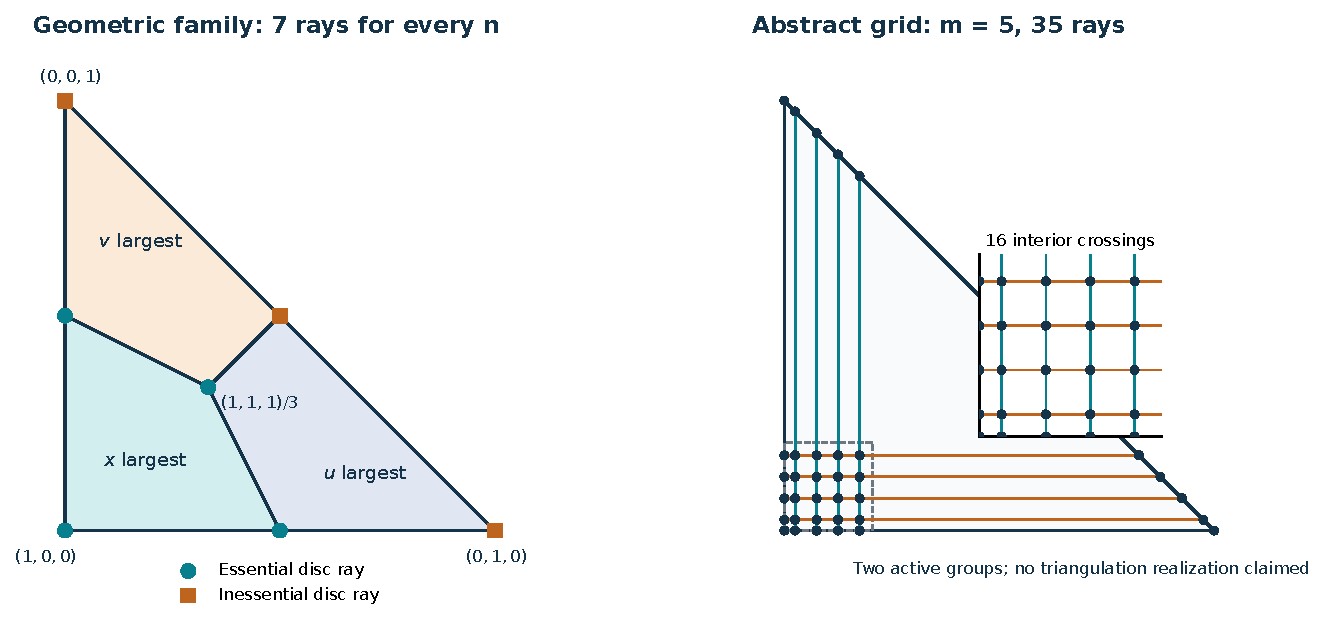
\includegraphics[width=.92\linewidth]{figures/minimum_diagrams.pdf}
\caption{Exact geometric models.  Left: the seven-vertex
two-cap diagram, drawn in the rescaled parameter section \(x+u+v=1\) with
\(u=y/A,\ v=z/A\).  Each region corresponds to the largest
of \(x,u,v\), or equivalently the active minimum after a
common affine shift.  Right: the abstract two-group grid
at \(m=5\), with \(m^2+2m=35\) vertices.  Only the left
diagram is asserted here to come from the exhibited
triangulated solid-torus family.}
\label{fig:diagrams}
\end{figure}

\subsection{Paired complete-enumeration timings}

The primary performance experiment uses \(n=1,2,4,8,16,32\)
base tetrahedra and \(t=n+2\) total tetrahedra.
For each size it retains a warmup and three paired rounds,
alternating the execution order.  The \emph{full} incumbent
arm builds the original kernel and enumerates with the
maintained automatic dispatcher; the full new arm builds
the sparse kernel and enumerates with the planar routine.
The dispatcher selects the old arrangement on this family.
Two additional arms use the \emph{same already constructed}
incumbent kernel, isolating enumeration after matching.

The timed task is complete ray-list exhaustion.  Full arms
include native geometry preparation, exact matching
construction, enumeration, and all native coordinate
checks performed during lifting.  Fixture generation,
shared-kernel setup, hashes, formula-vector comparison,
and serialization are outside the timers.  Disc-component
classification, independent coverage replay, sector
discovery, and whole-knot recognition are not timed here.
Every completed arm returns exactly the seven formula rays;
the old hyperplane, positive-direction, rejected-direction,
and pair-candidate counters match the all-size formulas.

% Generated from evidence/benchmark_summary.json; all times are milliseconds.
\begin{table}[htbp]
\centering
\small
\setlength{\tabcolsep}{3.8pt}
\begin{tabular}{r rrr rrr}
\toprule
& \multicolumn{3}{c}{Full construction and enumeration}
& \multicolumn{3}{c}{Enumeration on the same kernel} \\
\cmidrule(lr){2-4}\cmidrule(lr){5-7}
$n$ & Incumbent & Planar & Paired ratio & Incumbent & Planar & Paired ratio \\
\midrule
1 & 4.238 & 2.720 & 1.47 & 3.002 & 2.363 & 1.27 \\
2 & 8.550 & 3.057 & 2.83 & 8.224 & 2.898 & 2.84 \\
4 & 46.490 & 5.209 & 8.90 & 47.096 & 4.367 & 10.79 \\
8 & 537.411 & 8.730 & 61.64 & 530.946 & 6.916 & 73.80 \\
16 & 8\,572.669 & 19.861 & 482.82 & 8\,749.966 & 11.624 & 758.84 \\
32 & $40\,000$ cap & 48.458 & -- & $40\,000$ cap & 25.997 & -- \\
\bottomrule
\end{tabular}
\caption{Complete seven-ray enumeration for the double-capped Fibonacci family.
Times are medians of three alternating-order paired rounds, in milliseconds;
one warmup per arm is retained in the raw data and excluded from these medians.
Paired ratios are medians of within-round incumbent/planar time ratios,
not ratios of the displayed medians. For example, at $n=16$ the full paired
ratio is $482.82$, whereas the ratio of medians is $431.64$.
The two post-kernel arms receive exactly the same immutable incumbent-built kernel.
At $n=32$, all eight incumbent warmup/round runs reach the cooperative
$40\,000$\,ms cap after emitting seven rays but before proving enumeration
complete; the cap entries are allowances, not completed-run medians,
and no speed ratio is reported.}
\label{tab:planar-enumeration-benchmarks}
\end{table}

\begin{table}[htbp]
\centering
\small
\begin{tabular}{r rrrr}
\toprule
$n$ & Prior envelope (ms) & Planar (ms) & Paired prior/planar & Ratio of medians \\
\midrule
8 & 2.193 & 2.415 & 0.92 & 0.91 \\
32 & 8.534 & 8.741 & 0.97 & 0.98 \\
\bottomrule
\end{tabular}
\caption{Control against the earlier optimized nullity-two envelope enumerator,
loaded unmodified from the preceding research package. Both arms use the same
incumbent-built kernel and return the same three formula rays. Times are
medians of three paired rounds; values below one in either ratio column
indicate a slower planar implementation. These controls show no measured
advantage over the already optimized nullity-two method.}
\label{tab:planar-prior-envelope-control}
\end{table}

\begin{table}[htbp]
\centering
\small
\setlength{\tabcolsep}{4pt}
\begin{tabular}{r rrr rr}
\toprule
& \multicolumn{3}{c}{Complete construction (ms)}
& \multicolumn{2}{c}{Paired incumbent/sparse ratios} \\
\cmidrule(lr){2-4}\cmidrule(lr){5-6}
$k$ & Incumbent & Sparse once & Sparse reused & Reused source & Both cached \\
\midrule
1 & 72.133 & 81.463 & 8.004 & 8.84 & 1.88 \\
8 & 44.435 & 51.755 & 5.638 & 7.88 & 2.06 \\
32 & 61.126 & 64.297 & 12.041 & 4.74 & 2.02 \\
\bottomrule
\end{tabular}
\caption{Separate sparse-constructor measurements on supplied sparse sectors
of $t=1024$ layered solid tori. Times are medians of five paired rounds and
include unchanged exact rational elimination. The reused-source column
excludes its one-time preparation, while both ordinary single-call
constructors include preparation. The last column uses an additional control
where both constructors receive already validated geometry; it isolates
sparse kernel construction from validation reuse. Ratios are medians of
within-round ratios. The single-call sparse constructor is slower on these
cases. These are construction measurements, separate from complete ray
enumeration and from whole-knot recognition. All nine constructor cases
and every raw sample are retained in the data files.}
\label{tab:planar-sparse-source-control}
\end{table}


The \(n=32\) incumbent hits the cooperative 40-second
completion limit in both warmups and all six timed
incumbent rounds.  It has already emitted seven genuine
rays, but has not finished eliminating the other candidate
directions.  Its records are resource-limited, and no
speedup ratio is assigned to that size.  This is precisely
why the benchmark does not measure merely the time to
observe seven answers or the time to the first positive
disc.  A cooperative cap can overshoot by the duration
of an indivisible exact operation.

The rank-two control loads the preceding optimized
\code{sector\_envelope.py} unchanged and compares it with
the new method on the same kernel.  The older specialized
method is slightly faster in these measurements.  This
negative result argues for preserving the earlier branch
when designing an eventual dispatcher.  It would be
misleading to claim improvement over that method by
comparing only with an older all-equalities implementation.

\begin{figure}[htbp]
\centering
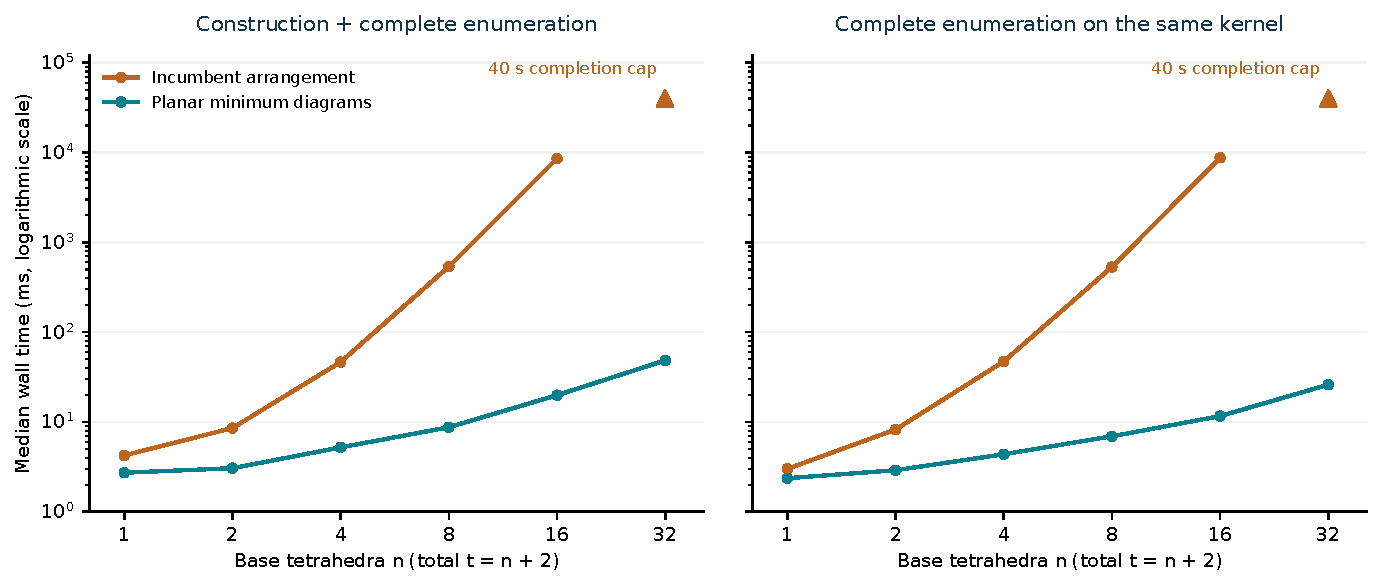
\includegraphics[width=.92\linewidth]{figures/paired_times.pdf}
\caption{Median complete-enumeration wall time over three
paired rounds, with logarithmic axes.  The incumbent
\(n=32\) value is a resource limit, displayed as a cap
marker rather than a completed timing.  These are
stage measurements on one growing family, not a fitted
worst-case exponent or a whole-recognizer speedup.}
\label{fig:times}
\end{figure}

\subsection{Construction-only reuse controls}

The separate sparse-constructor experiment uses nine
supplied-support cases on growing layered solid tori
and five rounds per case.  It distinguishes original
complete construction, one-shot sparse construction,
reused sparse construction, and a control in which
both constructors receive reusable prepared geometry.
Using ratios of median times across these cases, reused sparse construction is
1.38--9.01 times as fast as original complete construction.
When both reuse geometry, the measured ratio is
1.10--2.14.  One-shot sparse construction gives ratios
0.76--0.99 and is slower in this sample.

At \(t=1024,k=32\), original complete construction has
median 61.126 ms, one-shot sparse construction 64.297 ms,
and reused sparse construction 12.041 ms.  The matched
prepared-geometry control is 27.334 ms for the old builder
and 12.802 ms for the sparse builder.  Dense label entries
fall from 196,512 to 4,032.  This gives a concrete allocation
explanation while exposing the cost of preparing a
source that will be used only once.

All reported timings are observations from Python 3.12.14
in the supplied execution environment.  Exact source
digests, raw wall and CPU times where recorded, execution
order, counters, caps, and output hashes accompany the
package.  Three or five rounds on selected sources do
not support confidence claims about unrelated hardware
or a general input distribution.

\section{What is still required for quasi-polynomial recognition}
\label{sec:research}

The new theorem removes a local obstacle: a supplied sector of raw
matching dimension three has polynomially many relevant standard
rays, with a polynomial exact enumeration and coverage proof.
It does not bound how many sectors are required.  Even listing all
maximal quadrilateral choices gives \(3^t\) possible sectors, each
containing its own coordinate faces.  Polynomial work per selected
sector therefore remains compatible with exponential total work.
The fixed corpus demonstrates the utility of the new eligibility
class, not its completeness for all unknots.

The following conditional statement records exactly what the
local result can contribute.  It is the dimension-three extension
of the preceding report's complete-family accounting statement
~\cite{MinimumEnvelopes}; its point is to expose hypotheses, not to
claim they have been established.

\begin{corollary}[Conditional composition with a complete search]
\label{res:conditional}
Suppose a deterministic procedure on an \(n\)-crossing knot diagram
visits at most \(S(n)\) source-bound states and supplied sectors,
with the following properties:
\begin{enumerate}
\item all encoded state sizes, matching systems, and normal-vector
bit lengths are polynomial in \(n\);
\item each sector has matching nullity at most three, or is reduced
to one by a checked certificate preserving all relevant candidates;
\item every state construction, failed branch, restart, transition,
terminal decision, and certificate replay together costs
\(S(n)\poly(n)\);
\item the necessary essential-disc-component predicates can be
produced and independently replayed in polynomial bit time for
each emitted vector;
\item the certified source correspondence and selection theorem
guarantee that every unknot yields a relevant disc in at least one
enumerated ray, while the terminal rules justify the other outcome.
\end{enumerate}
Then the local enumeration, coverage replay, and disc tests can be
incorporated into a complete recognizer in \(S(n)\poly(n)\) bit time.
In particular, a quasi-polynomial bound on \(S(n)\) gives a
quasi-polynomial bound on this composed algorithm.
\end{corollary}
\begin{proof}
The planar output theorem gives polynomially many rays per eligible
sector.  Proposition~\ref{pl:operations}, the determinant bit bounds,
and the coverage-verification analysis give polynomial bit cost for
their exact generation and replay.  The fourth hypothesis supplies
the remaining polynomial work per ray.  The other hypotheses bound
all visited states and justify the two recognition conclusions.
Summing these costs over the entire search yields the stated bound.
\end{proof}

The fourth hypothesis is not shorthand for expanding every normal
disc.  Classical interval-orbit methods are polynomial in compressed
input parameters and can handle exponential normal
weight~\cite{AHT2006}.  The actual component predicate, its boundary
information, and its proof representation must satisfy the same
encoded-size accounting.  Likewise, efficient verification of an
essential hierarchy does not automatically give an efficient method
for discovering it.

If a strategy has polynomially many choices per level, a proved
\(O(\log n)\) depth leads to \(n^{O(\log n)}\) states.  Depth
\(O((\log n)^2)\) instead leads to \(n^{O((\log n)^2)}\).
A bound stated in the size of the latest triangulation is
insufficient if intermediate triangulations can grow without a
bound in the original \(n\).  A progress measure must also pay for
discarded suffixes and revisits, not only for successful cuts.

\subsection{Research questions with concrete success criteria}

The most useful next work should attack an unproved hypothesis or
remove an observed bottleneck.  The following questions are arranged
approximately in that order.

\paragraph{1. Constructive coverage by a small family of sectors.}
Can the search, under the actual knot-exterior hypotheses, generate
a quasi-polynomial family guaranteed to contain an essential-disc
standard ray whenever one exists?  A useful theorem must give the
selection procedure, its encoded cost, and a reason that some
witness survives.  An existential small support for a convenient
example is insufficient: layered meridians already show why support
cardinality alone is not a reliable universal parameter.  A first
manageable target is a natural restricted class of exteriors with
a certified reduction to sectors of effective cone dimension three.

\paragraph{2. Certified effective dimension above raw nullity three.}
Many raw kernel directions never meet the nonnegative orthant.
Can the active-face certificates of the recent incoming work
identify all coordinates that vanish on the feasible cone, then
produce a basis of its exact linear span without enumerating
high-dimensional candidate rays?  Once that span has dimension at
most three, the present geometry applies in it.  The missing
implementation should certify every removed direction and preserve
all feasible points.  Compare its cost with simply handling the
original sector; do not use a heuristic feasible support as proof
of a forced zero coordinate.

\paragraph{3. Incremental exact matching kernels.}
The sparse constructor eliminates the dense zero-label allocation,
but retains dense rational elimination.  Nearby sectors differ
by a few selected types.  Can one maintain a fraction-free
factorization, cycle basis, and source-bound rank certificate under
those changes?  A successful result should bound coefficient growth
and update cost, and should remain useful when a changed label
splits a previously contracted component.  The benchmark's
source-reuse improvement supplies a baseline; updates must be
compared against that stronger baseline.

\paragraph{4. Output-sensitive exact planar geometry.}
The present half-plane construction is deliberately elementary
and has a cubic worst-case arithmetic bound.  Can power-diagram
construction and an exact segment-overlay method reduce the
geometric stage toward \(O(k^2\log k)\), plus the unavoidable
cost of writing \(tR\) native coordinates?  A proof must count
clipping by the common source polygon without charging its
boundary once per irrelevant equality.  It must retain exact
behaviour for duplicate forms, lower-dimensional minima,
coincident edges, and a degenerate feasible section.

\paragraph{5. Genuine quadratic output or a stronger geometric bound.}
The abstract grid of Section~\ref{cf:grid} has
\(\Theta(p^2)\) rays, but its potential coefficients are not a
triangulation-realization theorem.  Does there exist a growing
family of valid compact knot exteriors or solid tori with
matching nullity three and \(\Omega(k^2)\) nonlink standard
rays in one sector?  Alternatively, does the sparse face-incidence
structure force a smaller bound?  Either outcome would sharpen
the parameter that the search should optimize.  The two-cap
family settles the single-group linear constant, not this
multi-group realization question.

\paragraph{6. Structural control of the active groups.}
The explicit bound separates \(A=\sum_v(m_v-1)\) from the
cross-group term.  Is it possible to simplify a triangulation,
choose a sector, or normalize a cut so that few vertex groups
have nontrivial minimum diagrams?  One nontrivial group removes
the quadratic crossing term entirely.  The quantity to preserve
is complete witness coverage, not merely the observed number of
cells in easy examples.  A candidate invariant should include
the cost and topological legality of the simplification.

\paragraph{7. A controlled extension to matching dimension four.}
For \(d=4\), the projective section is three-dimensional and
minimum cells are convex polyhedra.  Which diagram parameters
give a useful output bound for their common refinement?  A
general all-equalities arrangement is again too coarse.
Any extension should distinguish fixed dimension from
dimension growing with \(n\), handle non-simple intersections,
and provide a checkable coverage representation with a
bit-complexity proof.  Polynomiality for each fixed dimension
would still leave the global sector-selection problem open.

\paragraph{8. Smaller certificates and a formally checked geometric core.}
The current verifier reconstructs an uncontracted source model
for independence and can therefore be slower than the producer.
Can sparse elimination be certified by local row identities,
rank witnesses, and forest-potential equations, while retaining
independence from the producing algorithm?  Another useful
project is to formalize the canonical-lift correspondence,
planar Euler bound, and area-coverage theorem in Lean or another
proof assistant.  The acceptance criterion must rule out
artificial cell subdivisions as well as missing cells; area
alone without the distinct-label and dominance conditions
does not suffice.

\paragraph{9. Source-preserving compressed topology transitions.}
After a useful surface is chosen, can cutting and continuation
retain all ordered boundary attachments, coorientations, and
pattern data with polynomial encoded size?  The hierarchy
manuscript gives relevant compressed-cutting and certification
theorems~\cite{Lackenby2026}.  The implementation milestone
should be one complete transition with independently replayed
source and target objects.  Matching an aggregate boundary
profile is insufficient when different attachments produce
different topology.

\paragraph{10. A global amortized measure compatible with restarts.}
Can local batched descent, bounded trace search, and selected
normal cuts be charged to a single well-founded quantity with
only quasi-polynomially many values?  The value must account
for regluings, unsuccessful local searches, and invalidated
later hierarchy stages.  A lexicographic genus decrease proves
termination only after every coordinate bound and every
possible length have been quantified.  This is a principal
place where a genuine global asymptotic theorem could emerge.

\paragraph{11. Integration under a measured dispatcher.}
Which exact predicate should select the old specialized
rank-two envelope, the new planar method, and the general
fallback?  The new dimension-three path has a clear coverage
advantage; the lower-dimensional controls show why a universal
replacement is unwarranted.  A useful dispatcher experiment
should retain cold-start cost, preparation reuse, coverage
replay, and the full recognizer's time to a justified verdict.
It should include both unknots and nontrivial controls and
report every capped case.

\paragraph{12. Search-independent benchmark design.}
Can a benchmark suite be assembled before tuning the selection
policy, with independently regenerated complete ray oracles
where feasible and structural families beyond them?  Hold out
source families, not just individual supports of the same
triangulation.  Report distinct surfaces as well as repeated
sector occurrences.  Measure bit lengths, number of active
cells, overlay intersections, component-query work, memory,
and complete-exhaustion time.  The present package supplies
such measurements for a local stage, but does not estimate the
frequency of these sectors in an unbiased distribution of
hard knot diagrams.

\subsection{A concrete next milestone}

The next integration step can be made precise: combine a
source-bound exterior, certified effective-face reduction,
the appropriate complete envelope enumerator, and one
compressed topology transition, with all intermediate
certificates replayed by separate checkers.  Measure the
whole step and preserve the stronger incumbent branches.
In parallel, seek a theorem bounding how often that step
must be revisited.  The first task makes the local theorem
operational; the second determines whether it advances
the global quasi-polynomial programme beyond a faster
exponential search.

\section{Reproduction, package contents, and integration}
\label{sec:reproduce}

The package is self-contained for its default exact tests and
coverage replay.  It contains the full article source, rendered PDF,
vector figures, the new runtime modules, a pinned snapshot of their
maintained dependencies, focused tests, research drivers, a frozen
complete oracle, raw experimental evidence, and an additive patch
against the pinned repository commit.

\begin{center}
\small
\begin{tabularx}{\linewidth}{lX}
\toprule
Path & Contents and purpose\\
\midrule
\code{article/} & Main TeX, included sections, bibliography,
figures, tables, PDF, and figure-generation script.\\
\code{code/} & Standalone native package snapshot, research
drivers, selected fixtures, and the 39-test reproduction set.\\
\code{fixtures/} & Unchanged frozen complete discovery corpus
from the preceding minimum-envelope report.\\
\code{reference/} & Unmodified optimized rank-two envelope
module used as the stronger performance control.\\
\code{evidence/} & Full corpus results, compact summaries,
coverage certificates, replay outputs, family component
certificates, raw timings, and regression logs.\\
\code{scripts/} & Independent genuine/abstract differential
audit and sparse-constructor benchmark.\\
\code{integration.patch} & Additive repository changes;
unchanged dependency snapshots are not part of the patch.\\
\code{MANIFEST.json} & File sizes, SHA-256 digests, and
origin classification for every packaged file except itself.\\
\code{reproduce.py} & Manifest verification and isolated
reproduction commands.\\
\bottomrule
\end{tabularx}
\end{center}

From the package root, run
\begin{lstlisting}
python reproduce.py
\end{lstlisting}
This checks the manifest, runs the 31 new focused tests and eight
maintained sector-integration tests, and independently replays the
thirteen corpus and four family coverage certificates.  It writes
fresh output into a new reproduction directory.  It does not
overwrite the supplied evidence.

The longer computations are explicit options:
\begin{lstlisting}
python reproduce.py --audit --family --differential
python reproduce.py --fresh-regina
python reproduce.py --benchmark --sparse-benchmark
python reproduce.py --pdf
\end{lstlisting}
The first command repeats the full frozen-oracle audit, native
family census, and additional differential checks.  The second
also regenerates the designated complete Regina lists; it needs
Regina 7.4 or a compatible installation.  The third repeats the
paired timing protocol, including resource-limited incumbent runs.
The fourth compiles an isolated copy of the article using
\code{latexmk} and \code{pdflatex}.  Optional figure regeneration
uses Matplotlib.  The standard-library runtime checks do not
require either Regina or Matplotlib.

All raw experiment reports are preserved as produced, including
their original source paths and timestamps.  The executable
drivers accept explicit paths or locate their own package root;
they do not depend on those historical absolute paths.
The complete-output digest is a deterministic correctness target.
Wall-clock times, hardware behaviour, and PDF metadata are not
expected to reproduce bit-for-bit.  The manifest distinguishes
the new proposal from unchanged source copied for standalone use.

The patch adds the sparse constructor, planar producer, independent
checker, focused tests, and research drivers beneath
\path{Topology/UnknotRecognition/fast/}.  Before applying it to a
later revision, review any changes to the native source validator,
kernel representation, integer codec, and disc-certificate API.
The package's patch was checked against its exact base.  It does
not replace the maintained dispatcher or assign a new numbered
report in the repository's editorial structure.  The TeX article
and evidence can be filed according to the repository's intake
process.


\clearpage
\begin{thebibliography}{99}
\small
\setlength{\itemsep}{3pt}
\setlength{\parskip}{0pt}

\bibitem{Burton2009}
Benjamin A. Burton,
\emph{Converting between quadrilateral and standard solution sets
in normal surface theory},
Algebraic \& Geometric Topology 9 (2009), 2121--2174.
\href{https://doi.org/10.2140/agt.2009.9.2121}{doi:10.2140/agt.2009.9.2121}.
\url{https://arxiv.org/abs/0901.2629}.

\bibitem{Aurenhammer1987}
Franz Aurenhammer,
\emph{Power diagrams: properties, algorithms and applications},
SIAM Journal on Computing 16 (1987), 78--96.
\href{https://doi.org/10.1137/0216006}{doi:10.1137/0216006}.

\bibitem{Weibel2010}
Christophe Weibel,
\emph{Maximal f-vectors of Minkowski sums of large numbers of polytopes},
2010 preprint.
\url{https://arxiv.org/abs/1002.0155}.

\bibitem{Fogel2009}
Efi Fogel, Dan Halperin, and Christophe Weibel,
\emph{On the exact maximum complexity of Minkowski sums of convex polyhedra},
Discrete \& Computational Geometry 42 (2009), 654--669.
\href{https://doi.org/10.1007/s00454-009-9159-1}{doi:10.1007/s00454-009-9159-1}.

\bibitem{Burton2011}
Benjamin A. Burton,
\emph{Maximal admissible faces and asymptotic bounds for the normal
surface solution space},
Journal of Combinatorial Theory, Series A 118 (2011), 1410--1435.
\href{https://doi.org/10.1016/j.jcta.2010.12.011}{doi:10.1016/j.jcta.2010.12.011}.
\url{https://arxiv.org/abs/1004.2605}.

\bibitem{BurtonOzlen2012}
Benjamin A. Burton and Melih Ozlen,
\emph{A fast branching algorithm for unknot recognition with
experimental polynomial-time behaviour},
2012, revised 2014.
\url{https://arxiv.org/abs/1211.1079}.

\bibitem{AHT2006}
Ian Agol, Joel Hass, and William Thurston,
\emph{The computational complexity of knot genus and spanning area},
Transactions of the American Mathematical Society 358 (2006),
3821--3850.
\url{https://arxiv.org/abs/math/0205057}.

\bibitem{Lackenby2021}
Marc Lackenby,
\emph{Unknot recognition in quasi-polynomial time},
Oxford lecture handout, March 2021, especially slides 7 and 25.
\url{https://people.maths.ox.ac.uk/lackenby/quasipolynomial-talk-oxford-compressed.pdf}.

\bibitem{Lackenby2026}
Marc Lackenby,
\emph{Incompressible surfaces, hierarchies and unknot recognition},
25 July 2026, version 1.
\url{https://arxiv.org/abs/2607.23350v1}.

\bibitem{MinimumEnvelopes}
ProveIt research continuation,
\emph{Minimum Envelopes and Complete Normal-Surface Sectors},
incoming package \texttt{unknot\_minimum\_envelopes\_20261009.zip},
9 October 2026.  Repository location:
\path{docs/incoming/unknot_minimum_envelopes_20261009.zip},
at commit \texttt{\basecommit}.

\bibitem{ActiveFaces}
ProveIt research continuation,
\emph{Active faces and batched descent},
incoming package
\path{docs/incoming/unknot_active_faces_batched_descent_20261009.zip},
9 October 2026, at the same pinned commit.

\bibitem{TraceSearch}
ProveIt research continuation,
\emph{Trace search},
incoming package
\path{docs/incoming/unknot_trace_search_20261009.zip},
9 October 2026, at the same pinned commit.

\bibitem{CycleKernels}
ProveIt research continuation,
\emph{Cycle-envelope kernels},
incoming package
\path{docs/incoming/ProveIt_Cycle_Envelope_Kernels_20261009.zip},
9 October 2026, at the same pinned commit.

\bibitem{RootedDiscs}
ProveIt research continuation,
\emph{Rooted disc components},
incoming package
\path{docs/incoming/ProveIt_Rooted_Disc_Components_2026-10-09.zip},
9 October 2026, at the same pinned commit.

\bibitem{AffineProfiles}
ProveIt research continuation,
\emph{Affine orbit profiles},
incoming package
\path{docs/incoming/ProveIt_Affine_Orbit_Profiles_2026-10-09.zip},
9 October 2026, at the same pinned commit.

\end{thebibliography}

\end{document}
